\documentclass{article}\usepackage[]{graphicx}\usepackage[]{color}
%% maxwidth is the original width if it is less than linewidth
%% otherwise use linewidth (to make sure the graphics do not exceed the margin)
\makeatletter
\def\maxwidth{ %
  \ifdim\Gin@nat@width>\linewidth
    \linewidth
  \else
    \Gin@nat@width
  \fi
}
\makeatother

\definecolor{fgcolor}{rgb}{0.345, 0.345, 0.345}
\newcommand{\hlnum}[1]{\textcolor[rgb]{0.686,0.059,0.569}{#1}}%
\newcommand{\hlstr}[1]{\textcolor[rgb]{0.192,0.494,0.8}{#1}}%
\newcommand{\hlcom}[1]{\textcolor[rgb]{0.678,0.584,0.686}{\textit{#1}}}%
\newcommand{\hlopt}[1]{\textcolor[rgb]{0,0,0}{#1}}%
\newcommand{\hlstd}[1]{\textcolor[rgb]{0.345,0.345,0.345}{#1}}%
\newcommand{\hlkwa}[1]{\textcolor[rgb]{0.161,0.373,0.58}{\textbf{#1}}}%
\newcommand{\hlkwb}[1]{\textcolor[rgb]{0.69,0.353,0.396}{#1}}%
\newcommand{\hlkwc}[1]{\textcolor[rgb]{0.333,0.667,0.333}{#1}}%
\newcommand{\hlkwd}[1]{\textcolor[rgb]{0.737,0.353,0.396}{\textbf{#1}}}%

\usepackage{framed}
\makeatletter
\newenvironment{kframe}{%
 \def\at@end@of@kframe{}%
 \ifinner\ifhmode%
  \def\at@end@of@kframe{\end{minipage}}%
  \begin{minipage}{\columnwidth}%
 \fi\fi%
 \def\FrameCommand##1{\hskip\@totalleftmargin \hskip-\fboxsep
 \colorbox{shadecolor}{##1}\hskip-\fboxsep
     % There is no \\@totalrightmargin, so:
     \hskip-\linewidth \hskip-\@totalleftmargin \hskip\columnwidth}%
 \MakeFramed {\advance\hsize-\width
   \@totalleftmargin\z@ \linewidth\hsize
   \@setminipage}}%
 {\par\unskip\endMakeFramed%
 \at@end@of@kframe}
\makeatother

\definecolor{shadecolor}{rgb}{.97, .97, .97}
\definecolor{messagecolor}{rgb}{0, 0, 0}
\definecolor{warningcolor}{rgb}{1, 0, 1}
\definecolor{errorcolor}{rgb}{1, 0, 0}
\newenvironment{knitrout}{}{} % an empty environment to be redefined in TeX

\usepackage{alltt}
\usepackage[sc]{mathpazo}
\usepackage[T1]{fontenc}
\usepackage{geometry}
\usepackage[utf8]{inputenc}
\usepackage{amsmath}
\usepackage{float}
\usepackage{caption}
\usepackage{subcaption}
\usepackage[demo]{graphicx}
\usepackage{booktabs}
\geometry{verbose,tmargin=2.5cm,bmargin=2.5cm,lmargin=2.5cm,rmargin=2.5cm}
\setcounter{secnumdepth}{2}
\setcounter{tocdepth}{2}
\usepackage{url}
\usepackage[unicode=true,pdfusetitle,
 bookmarks=true,bookmarksnumbered=true,bookmarksopen=true,bookmarksopenlevel=2,
 breaklinks=false,pdfborder={0 0 1},backref=false,colorlinks=false]
 {hyperref}
\hypersetup{
 pdfstartview={XYZ null null 1}}
\usepackage{breakurl}
\usepackage{array}
\newcommand\Mark[1]{\textsuperscript#1}
\renewcommand{\hlcom}[1]{\textcolor[rgb]{0.678,0.584,0.686}{\textbf{#1}}}%
\IfFileExists{upquote.sty}{\usepackage{upquote}}{}
\begin{document}



\begingroup
\centering
{\LARGE Predicting the Chromatin Conformation From ChIPseq CebpE: part 1 (Component Analysis) \\[1.5em]
\large Ricky Lim\Mark{1}, Samuel Collombet\Mark{2}, Agus Salim\Mark{3}, Touati Benoukraf\Mark{1}}\\[1em]
\begin{tabular}{*{3}{>{\centering}p{.25\textwidth}}}
    \Mark{1}Cancer Science Institute of Singapore, National University of Singapore&\Mark{2}Institut de Biologie de l'Ecole Normale Superieur de Paris& \Mark{3}Department of Mathematics and Statistics& \tabularnewline
%National University of Singapore& La Trobe University& National University of Singapore\tabularnewline
%\url{csilr@nus.edu.sg} & \url{samuel.collombet@ens.fr} & \url{A.Salim@latrobe.edu.au} & \url{csitb@nus.edu.sg}
\url{benoukraf@nus.edu.sg}
\end{tabular}\par
\endgroup

\begin{knitrout}
\definecolor{shadecolor}{rgb}{0.969, 0.969, 0.969}\color{fgcolor}\begin{kframe}
\begin{alltt}
\hlkwd{source}\hlstd{(}\hlstr{'/home/ricky/Rlim/ChromatinConformation/ComponentCalls/ComponentCalls.R'}\hlstd{)}
\hlstd{work_dir} \hlkwb{=} \hlstr{'/home/ricky/Rlim/ChromatinConformation/ComponentCalls/CebpE/'}
\end{alltt}
\end{kframe}
\end{knitrout}

\section{Load Dataset}
Proof-of-concept: We used ChIP-seq peak signals of CebpE in bone marrow cells from Koeffler's Lab.
Here is the quick insight on Cebp Protein from \href{https://pubmedylicious.appspot.com/result/564730861610598://pubmedylicious.appspot.com/result/5073520312713216}{Pubmedylicious}.

\begin{knitrout}
\definecolor{shadecolor}{rgb}{0.969, 0.969, 0.969}\color{fgcolor}\begin{kframe}
\begin{alltt}
\hlstd{Koeffler_BM_CebpE} \hlkwb{<-} \hlkwd{read.table}\hlstd{(}\hlkwd{paste0}\hlstd{(work_dir,}
                        \hlstr{'Input/KoefflerLab_BM_ChIPseq_CebpE_mm10_q10rmdup_peaks.xls'}\hlstd{),}
                        \hlkwc{header}\hlstd{=T,} \hlkwc{sep}\hlstd{=}\hlstr{'\textbackslash{}t'}\hlstd{,} \hlkwc{row.names}\hlstd{=}\hlnum{10}\hlstd{,} \hlkwc{skip}\hlstd{=}\hlnum{28}\hlstd{)}

\hlstd{p1} \hlkwb{<-} \hlkwd{ggplot}\hlstd{(Koeffler_BM_CebpE,} \hlkwd{aes}\hlstd{(}\hlkwc{x}\hlstd{=pileup))} \hlopt{+}
        \hlkwd{geom_histogram}\hlstd{(}\hlkwd{aes}\hlstd{(}\hlkwc{y} \hlstd{= ..density..),} \hlkwc{fill}\hlstd{=}\hlstr{'#969696'}\hlstd{,} \hlkwc{binwidth}\hlstd{=}\hlnum{25}\hlstd{)} \hlopt{+}
        \hlkwd{geom_line}\hlstd{(}\hlkwc{stat}\hlstd{=}\hlstr{'density'}\hlstd{,} \hlkwc{alpha}\hlstd{=}\hlnum{0.5}\hlstd{,} \hlkwc{size}\hlstd{=}\hlnum{1.5}\hlstd{)} \hlopt{+}
        \hlkwd{scale_x_continuous}\hlstd{(}\hlkwc{breaks}\hlstd{=}\hlkwd{seq}\hlstd{(}\hlnum{0}\hlstd{,}\hlnum{450}\hlstd{,} \hlnum{25}\hlstd{))} \hlopt{+}
        \hlkwd{ggtitle}\hlstd{(}\hlstr{'Distribution of ChIP-seq Peaks (Koeffler_BM_CebpE)'}\hlstd{)}\hlopt{+}
        \hlkwd{xlab}\hlstd{(}\hlstr{'Score'}\hlstd{)}
\hlkwd{ggsave}\hlstd{(}\hlstr{'figs/Koeffler_BM_CebpE_CountChipSeqPeaks.pdf'}\hlstd{, p1)}
\end{alltt}


{\ttfamily\noindent\itshape\color{messagecolor}{\#\# Saving 7 x 7 in image}}\end{kframe}
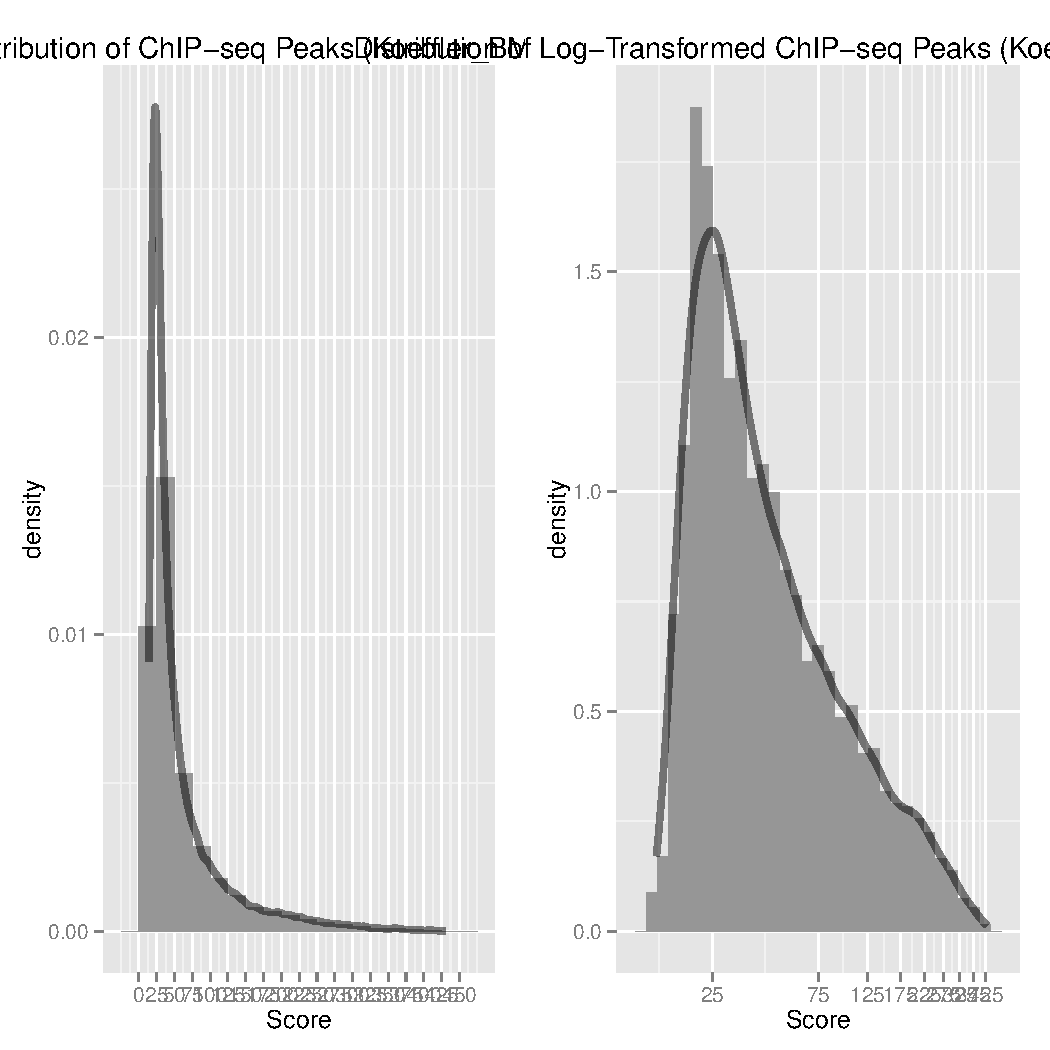
\includegraphics[width=\maxwidth]{figure/Dataset} 
\begin{kframe}\begin{alltt}
\hlcom{#summary(Koeffler_BM_CebpE$pileup)}
\hlcom{#summary(log10(Koeffler_BM_CebpE$pileup))}
\hlstd{p2} \hlkwb{<-} \hlkwd{ggplot}\hlstd{(Koeffler_BM_CebpE,} \hlkwd{aes}\hlstd{(}\hlkwc{x}\hlstd{=pileup))} \hlopt{+}
        \hlkwd{geom_histogram}\hlstd{(}\hlkwd{aes}\hlstd{(}\hlkwc{y} \hlstd{= ..density..),} \hlkwc{fill}\hlstd{=}\hlstr{'#969696'}\hlstd{,} \hlkwc{binwidth}\hlstd{=}\hlnum{.05}\hlstd{)} \hlopt{+}
        \hlkwd{geom_line}\hlstd{(}\hlkwc{stat}\hlstd{=}\hlstr{'density'}\hlstd{,} \hlkwc{alpha}\hlstd{=}\hlnum{0.5}\hlstd{,} \hlkwc{size}\hlstd{=}\hlnum{1.5}\hlstd{)} \hlopt{+}
        \hlkwd{scale_x_log10}\hlstd{(}\hlkwc{breaks}\hlstd{=}\hlkwd{seq}\hlstd{(}\hlnum{25}\hlstd{,}\hlnum{450}\hlstd{,} \hlnum{50}\hlstd{))} \hlopt{+}
        \hlkwd{ggtitle}\hlstd{(}\hlstr{'Distribution of Log-Transformed ChIP-seq Peaks (Koeffler_BM_CebpE)'}\hlstd{)} \hlopt{+}
        \hlkwd{xlab}\hlstd{(}\hlstr{'Score'}\hlstd{)}
\hlkwd{ggsave}\hlstd{(}\hlstr{'figs/Koeffler_BM_CebpE_CountChipSeqPeaks_log.pdf'}\hlstd{, p2)}
\end{alltt}


{\ttfamily\noindent\itshape\color{messagecolor}{\#\# Saving 20 x 12.2 in image}}\begin{alltt}
\hlcom{#grid.arrange(p1, p2, ncol=2)}
\hlcom{#p <- arrangeGrob(p1,p2, ncol=2)}
\hlcom{#ggsave('figs/Koeffler_BM_CebpE_CountChipSeqPeaks.pdf', p)}
\end{alltt}
\end{kframe}
\end{knitrout}

\clearpage
\begin{figure}[!htbp]
    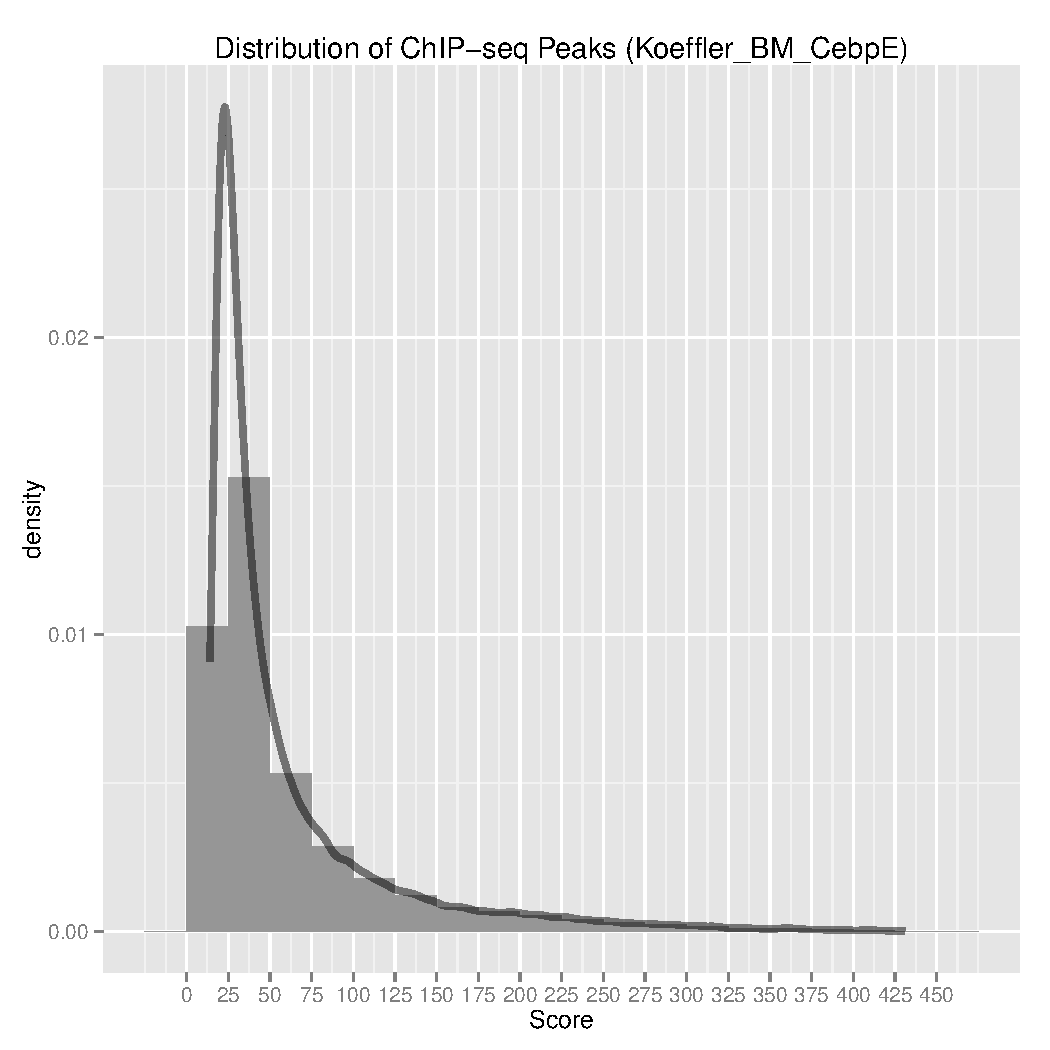
\includegraphics[width=6in, height=3in]{figs/Koeffler_BM_CebpE_CountChipSeqPeaks.pdf}
    \\
    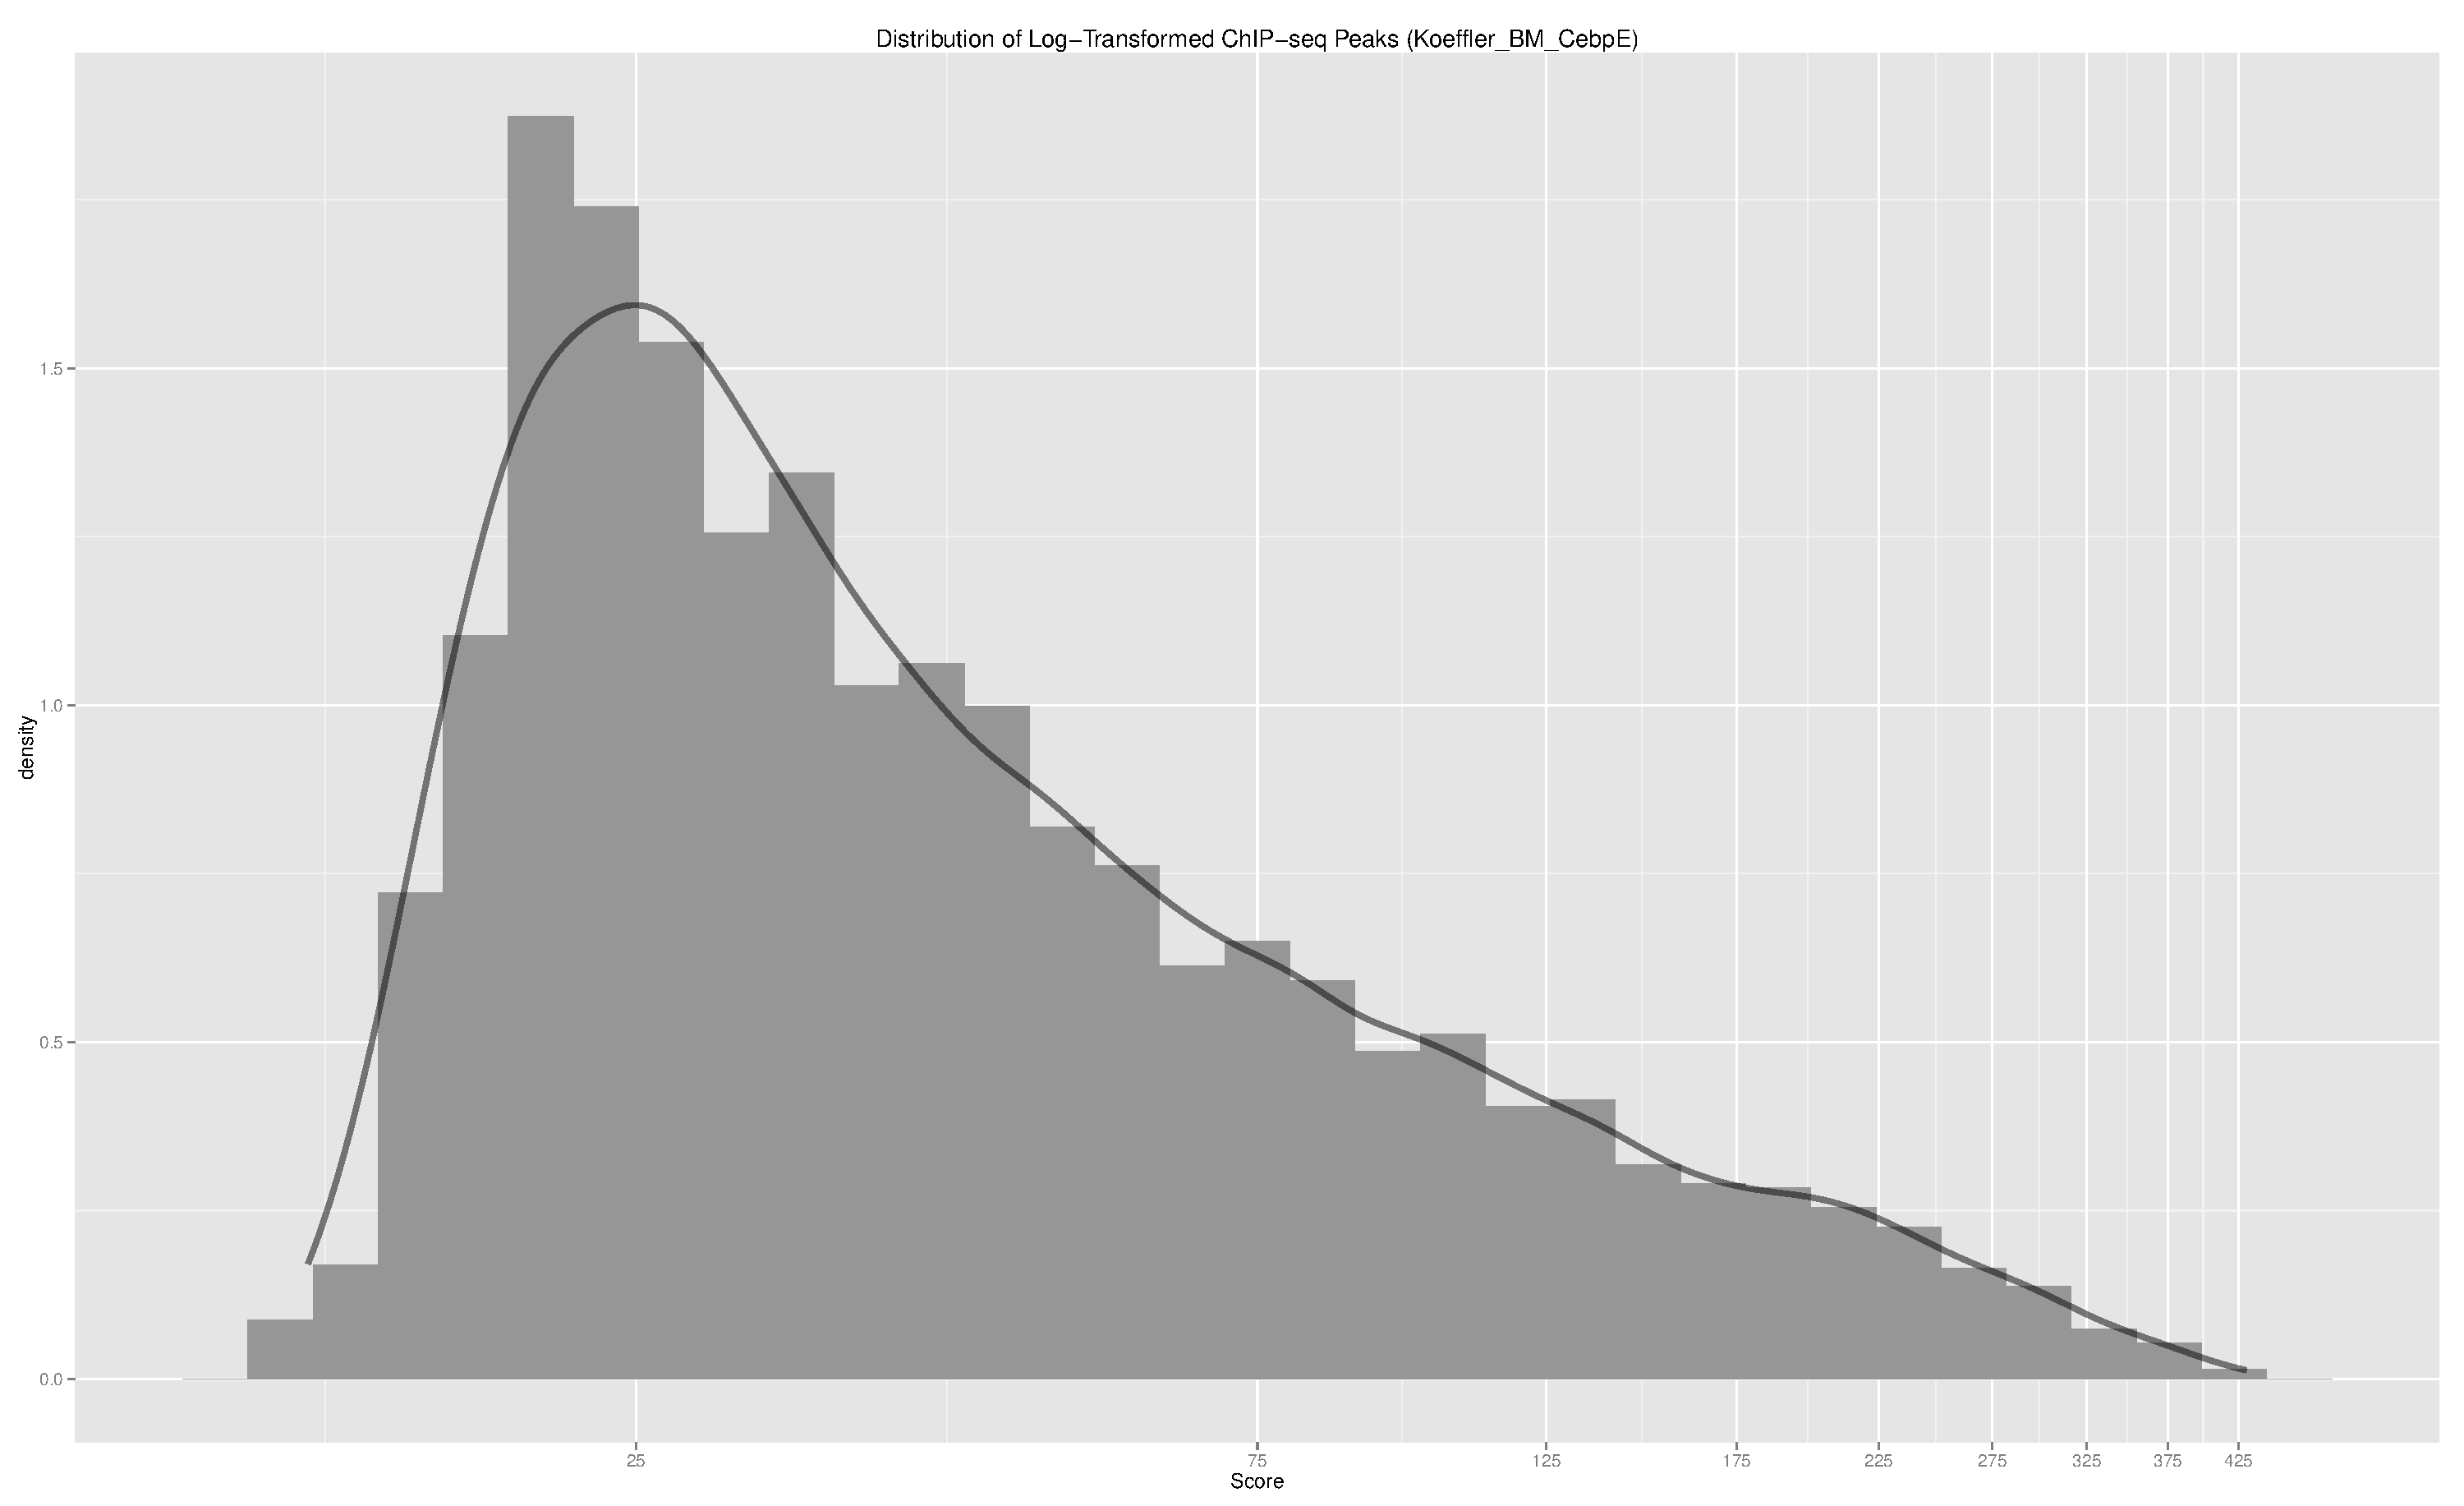
\includegraphics[width=6in, height=3in]{figs/Koeffler_BM_CebpE_CountChipSeqPeaks_log.pdf}
    \caption{Distibution of ChIPseq Peak Pileup Scores.}
    \label{fig:DistributionChipPeak}
\end{figure}
\clearpage

\section{Models Fitted on ChIP-seq Peaks}
Here, we attempt to fit ChIP-seq peaks with Normal, and Negative Binomial distributions. 
Figure ~\ref{fig:modelFitting} demonstrates that Negative Binomial distribution provides better fit with higher loglik (-4978.32), compared to normal distribution with lower loglik of -5429.51.   

\begin{knitrout}
\definecolor{shadecolor}{rgb}{0.969, 0.969, 0.969}\color{fgcolor}\begin{kframe}
\begin{alltt}
\hlkwd{library}\hlstd{(MASS)}

\hlkwd{set.seed}\hlstd{(}\hlnum{123}\hlstd{)}
\hlstd{chip_data} \hlkwb{<-} \hlkwd{sort}\hlstd{(}\hlkwd{sample}\hlstd{(Koeffler_BM_CebpE}\hlopt{$}\hlstd{pileup,} \hlnum{1000}\hlstd{))}
\hlstd{n} \hlkwb{<-} \hlkwd{length}\hlstd{(chip_data)}

\hlcom{# fitting with models}
\hlstd{normal.par} \hlkwb{<-} \hlkwd{fitdistr}\hlstd{(chip_data,} \hlstr{'normal'}\hlstd{)}
\hlstd{poisson.par} \hlkwb{<-} \hlkwd{fitdistr}\hlstd{(chip_data,} \hlstr{'Poisson'}\hlstd{)}
\hlstd{negbi.par} \hlkwb{<-} \hlkwd{fitdistr}\hlstd{(chip_data,} \hlstr{'negative binomial'}\hlstd{)}

\hlcom{# counts estimates generated by models}
\hlstd{normal.estimate} \hlkwb{<-} \hlkwd{rnorm}\hlstd{(n, normal.par}\hlopt{$}\hlstd{estimate)}
\hlstd{poisson.estimate} \hlkwb{<-} \hlkwd{rpois}\hlstd{(n, poisson.par}\hlopt{$}\hlstd{estimate)}
\hlstd{negbi.estimate} \hlkwb{<-} \hlkwd{rnbinom}\hlstd{(n,} \hlkwc{size}\hlstd{=negbi.par}\hlopt{$}\hlstd{estimate[}\hlstr{'size'}\hlstd{],} \hlkwc{mu}\hlstd{=negbi.par}\hlopt{$}\hlstd{estimate[}\hlstr{'mu'}\hlstd{])}
\end{alltt}
\end{kframe}
\end{knitrout}

\begin{knitrout}
\definecolor{shadecolor}{rgb}{0.969, 0.969, 0.969}\color{fgcolor}
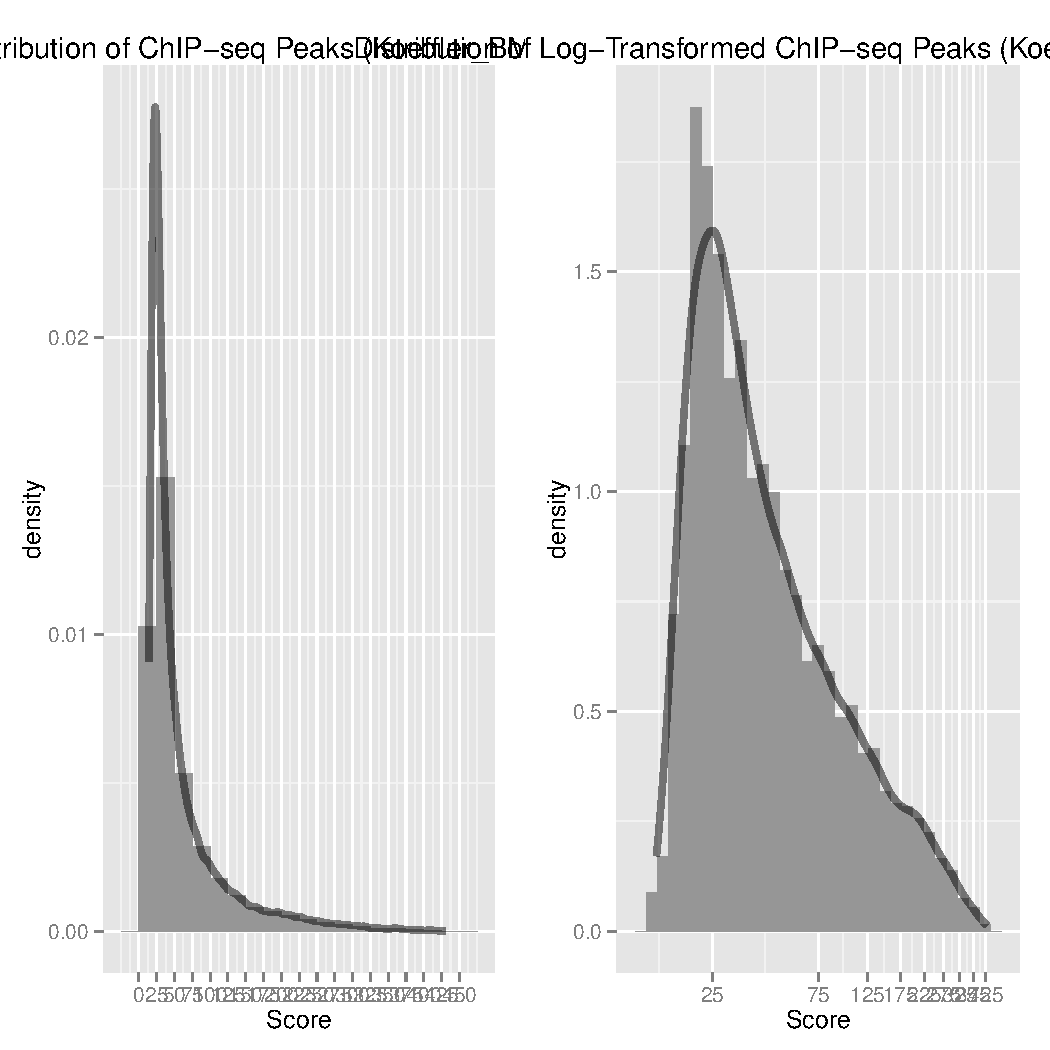
\includegraphics[width=\maxwidth]{figure/PlotModelFits} 
\begin{kframe}\begin{verbatim}
## X11cairo 
##        2
## X11cairo 
##        2
## X11cairo 
##        2
\end{verbatim}
\end{kframe}
\end{knitrout}

\begin{figure}[!htp]
    \centering
    \subfloat{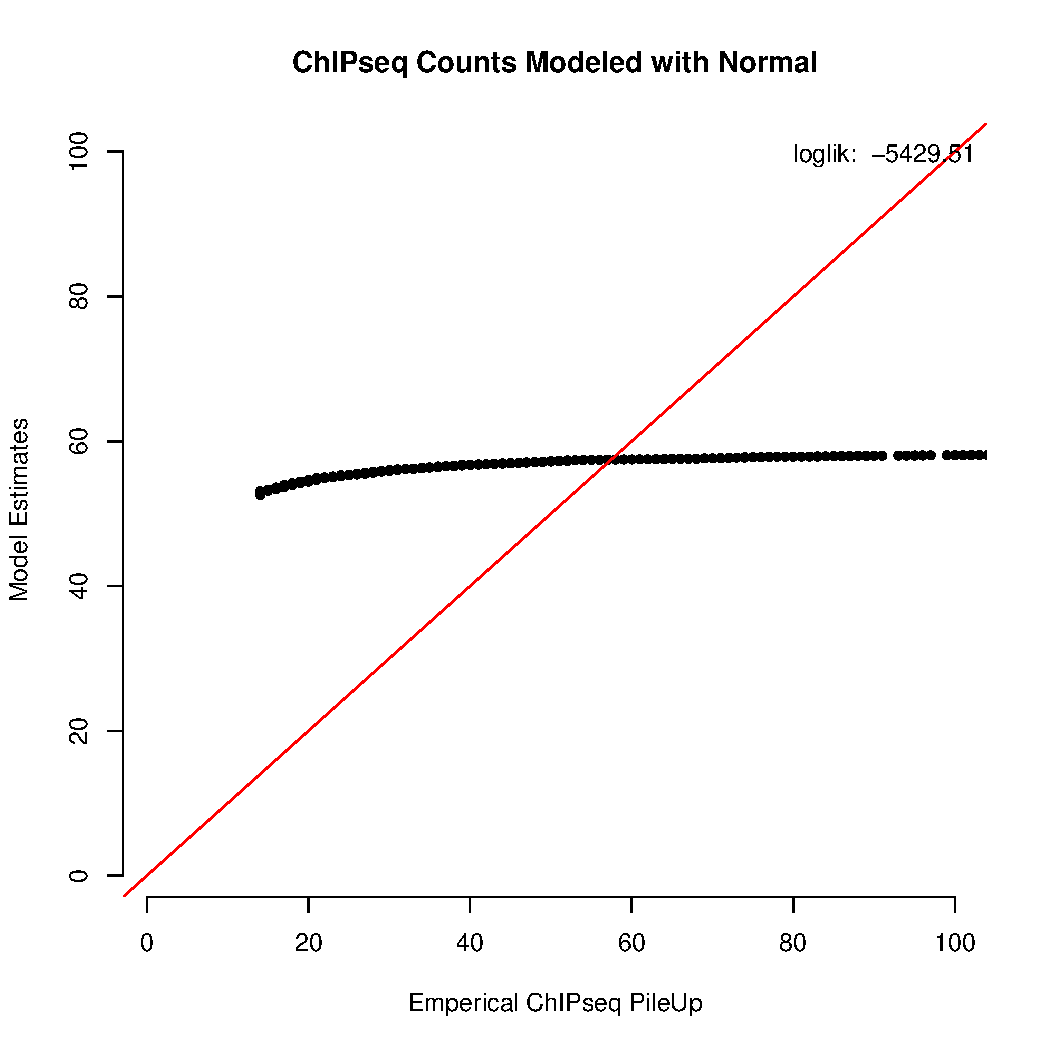
\includegraphics[width = 2in]{figs/Koeffler_BM_CebpE_normalModel.pdf}}
    %\subfloat{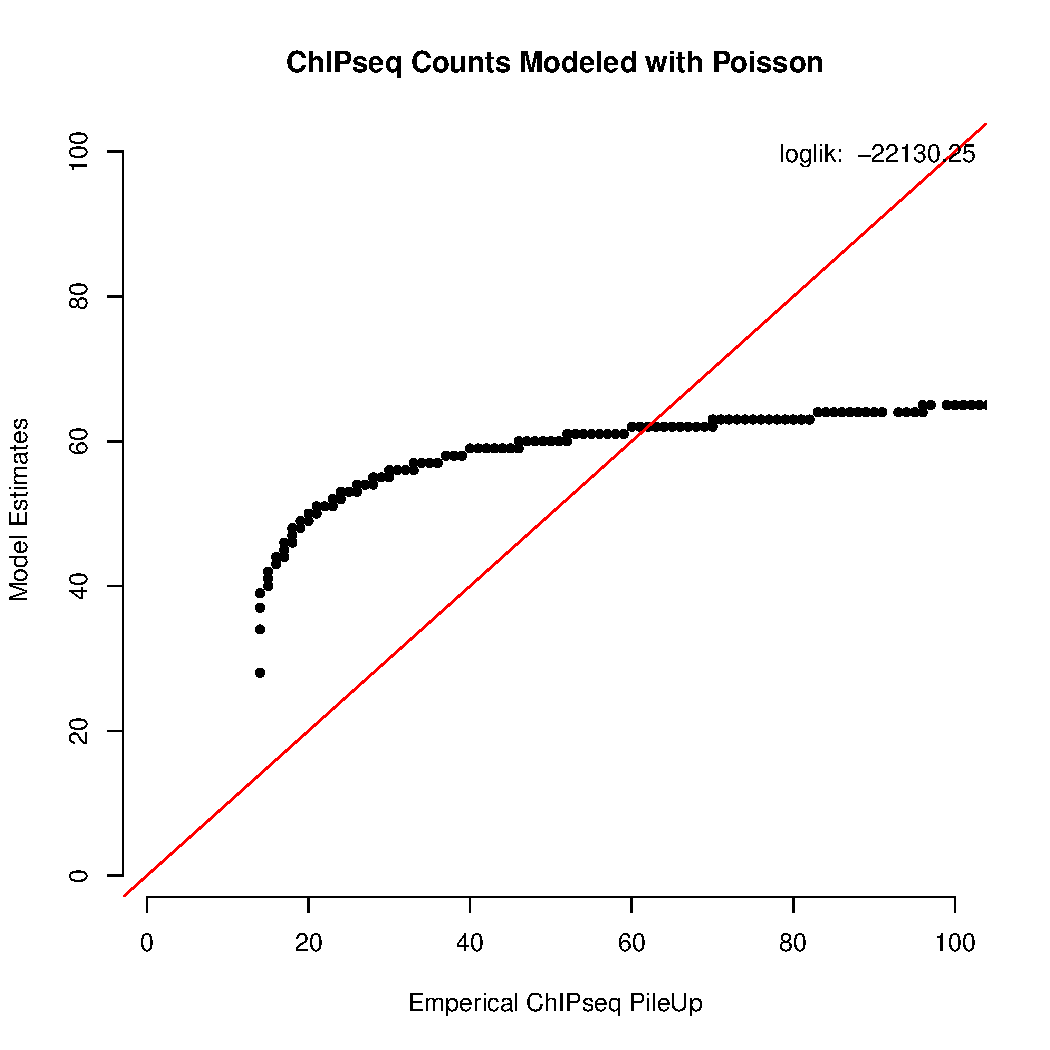
\includegraphics[width = 2in]{ComponentCalls/CebpE/Output/Plots/Koeffler_BM_CebpE_poissonModel.pdf}}
    \subfloat{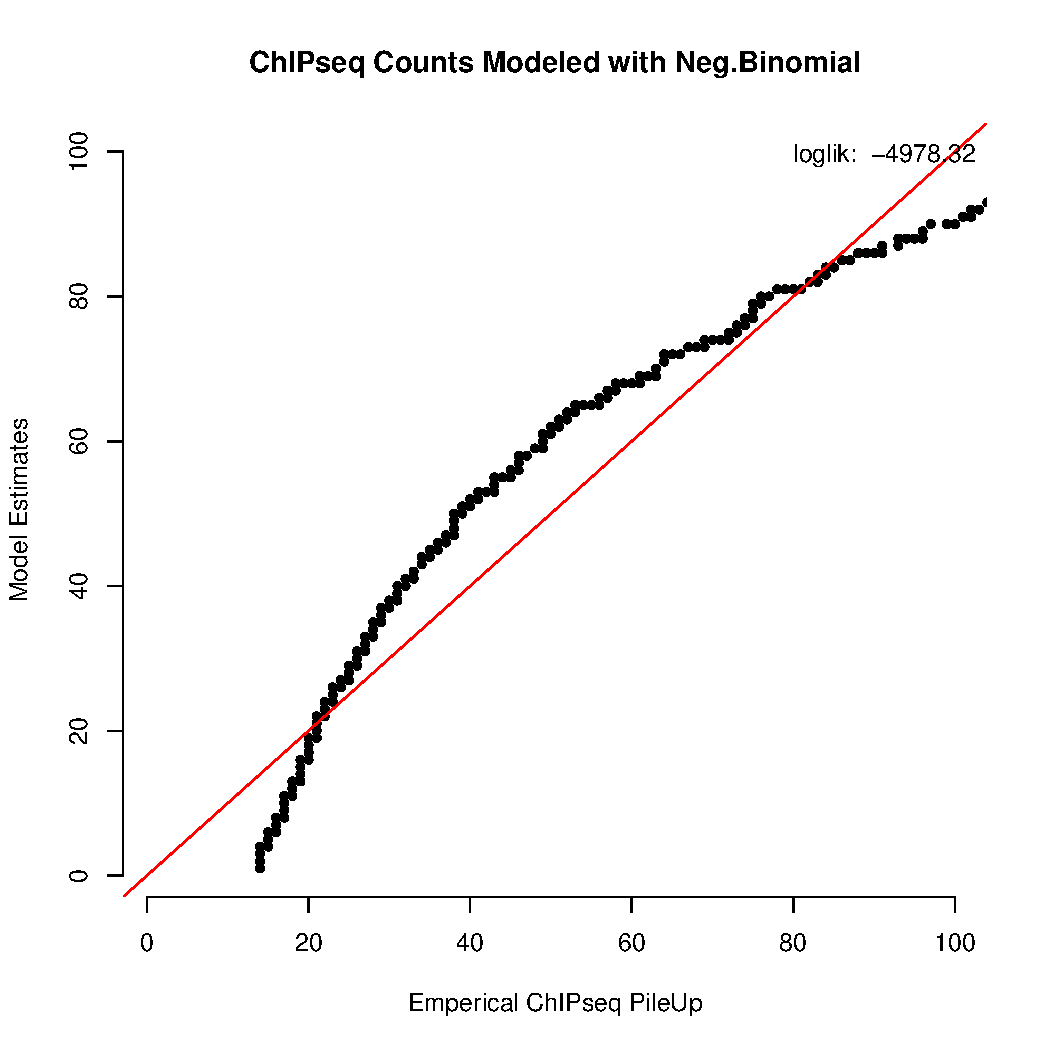
\includegraphics[width = 2in]{figs/Koeffler_BM_CebpE_negBinomModel.pdf}}
    \caption{Models Fitting: normal, and neg.binomial. 
             The perfect fit is drawn on the red line, in which the model estimates match perfectly to the empirical observation. 
             The more points lying on this line, the better the fit.
             }
    \label{fig:modelFitting}
\end{figure}
\clearpage

\section{Mixture Models Fitted on ChIP-seq Peaks}

Figure ~\ref{fig:modelFitting} shows that single model is not sufficient to fit the ChIPseq data. 
For this reason, here we fit the mixture models of Normal (Gaussian Mixture Models or GMM) and Negative Binomial distributions (Negative Binomial Models or NBMs). 

\subsection{GMMs Fitted on ChIP-seq Peaks}

\begin{knitrout}
\definecolor{shadecolor}{rgb}{0.969, 0.969, 0.969}\color{fgcolor}\begin{kframe}
\begin{alltt}
\hlcom{# fit with several k-component-GMMs}
\hlstd{GMMs_list_Koeffler_BM_CebpE} \hlkwb{<-} \hlkwd{fitMMs}\hlstd{(}\hlkwc{X}\hlstd{=Koeffler_BM_CebpE}\hlopt{$}\hlstd{pileup,} \hlkwc{max_k}\hlstd{=}\hlnum{10}\hlstd{,} \hlkwc{model} \hlstd{=} \hlstr{'GMM'}\hlstd{)}
\end{alltt}
\end{kframe}
\end{knitrout}

\subsection{NBMs fitted on ChIPseq Peaks}

\begin{knitrout}
\definecolor{shadecolor}{rgb}{0.969, 0.969, 0.969}\color{fgcolor}\begin{kframe}
\begin{alltt}
\hlstd{NBMs_list_Koeffler_BM_CebpE} \hlkwb{<-} \hlkwd{fitMMs}\hlstd{(}\hlkwc{X}\hlstd{=Koeffler_BM_CebpE}\hlopt{$}\hlstd{pileup,} \hlkwc{max_k}\hlstd{=}\hlnum{10}\hlstd{,} \hlstr{'NBM'}\hlstd{)}
\end{alltt}
\end{kframe}
\end{knitrout}

%\subsubsection{Model Parameters}


\section{Visualization of the Fitted MMs on ChIP-seq distributions}

\subsection{Fitted GMMs Visualized on ChiP-seq distributions}
\begin{knitrout}
\definecolor{shadecolor}{rgb}{0.969, 0.969, 0.969}\color{fgcolor}\begin{kframe}
\begin{alltt}
\hlkwd{visualizeFitMMs}\hlstd{(}\hlkwc{X}\hlstd{=Koeffler_BM_CebpE,} \hlkwc{MMs_list}\hlstd{=GMMs_list_Koeffler_BM_CebpE,}
                \hlkwc{max_k}\hlstd{=}\hlnum{10}\hlstd{,} \hlkwc{output_n}\hlstd{=}\hlstr{'figs/Koeffler_BM_CebpE_GMM_ModelVisualization'}\hlstd{,}
                \hlkwc{model} \hlstd{=} \hlstr{'GMM'}\hlstd{,} \hlkwc{titleName}\hlstd{=}\hlstr{'Koeffler_BM_CebpE'}\hlstd{)}
\end{alltt}
\end{kframe}
\end{knitrout}

\begin{figure}[!htp]
    \centering
    \subfloat{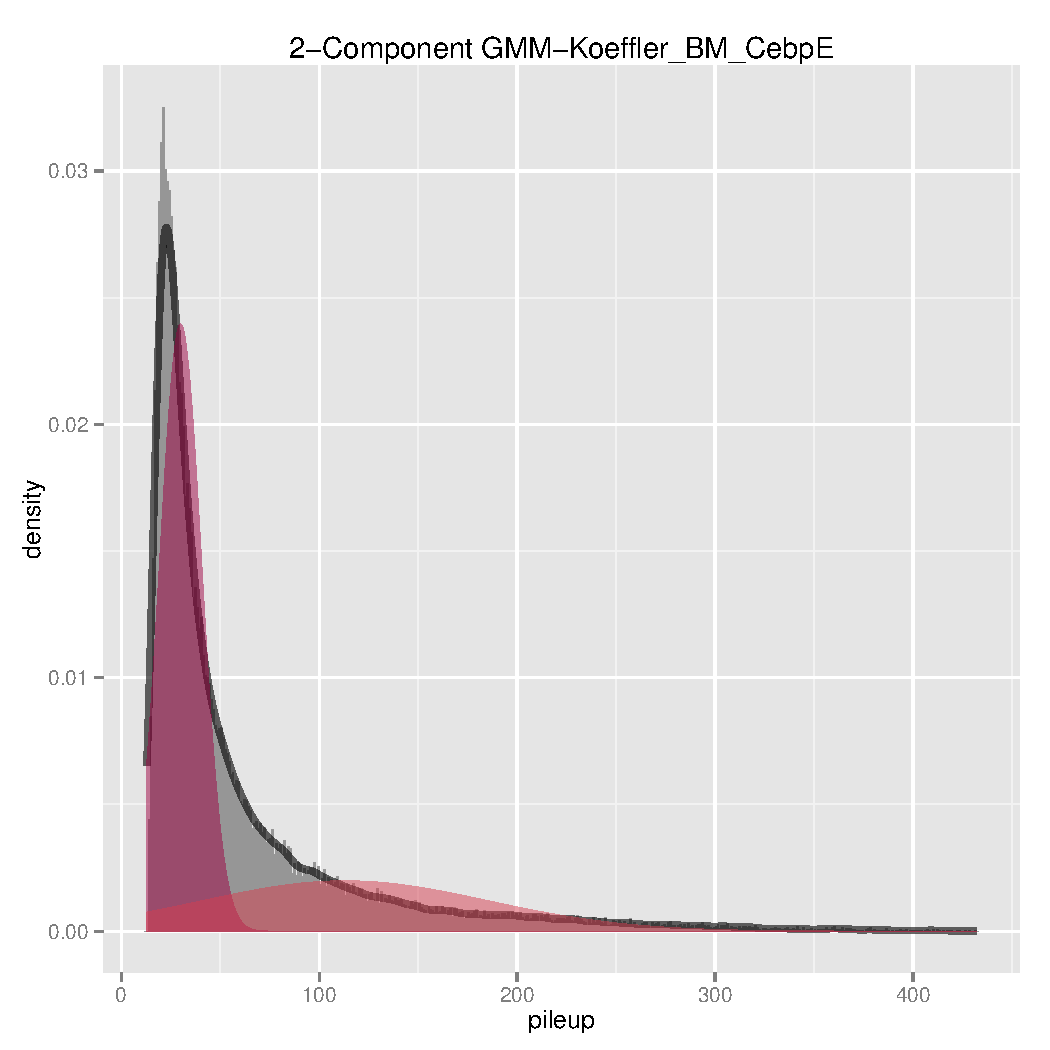
\includegraphics[width = 2in]{figs/Koeffler_BM_CebpE_GMM_ModelVisualization_comp2.pdf}}
    \subfloat{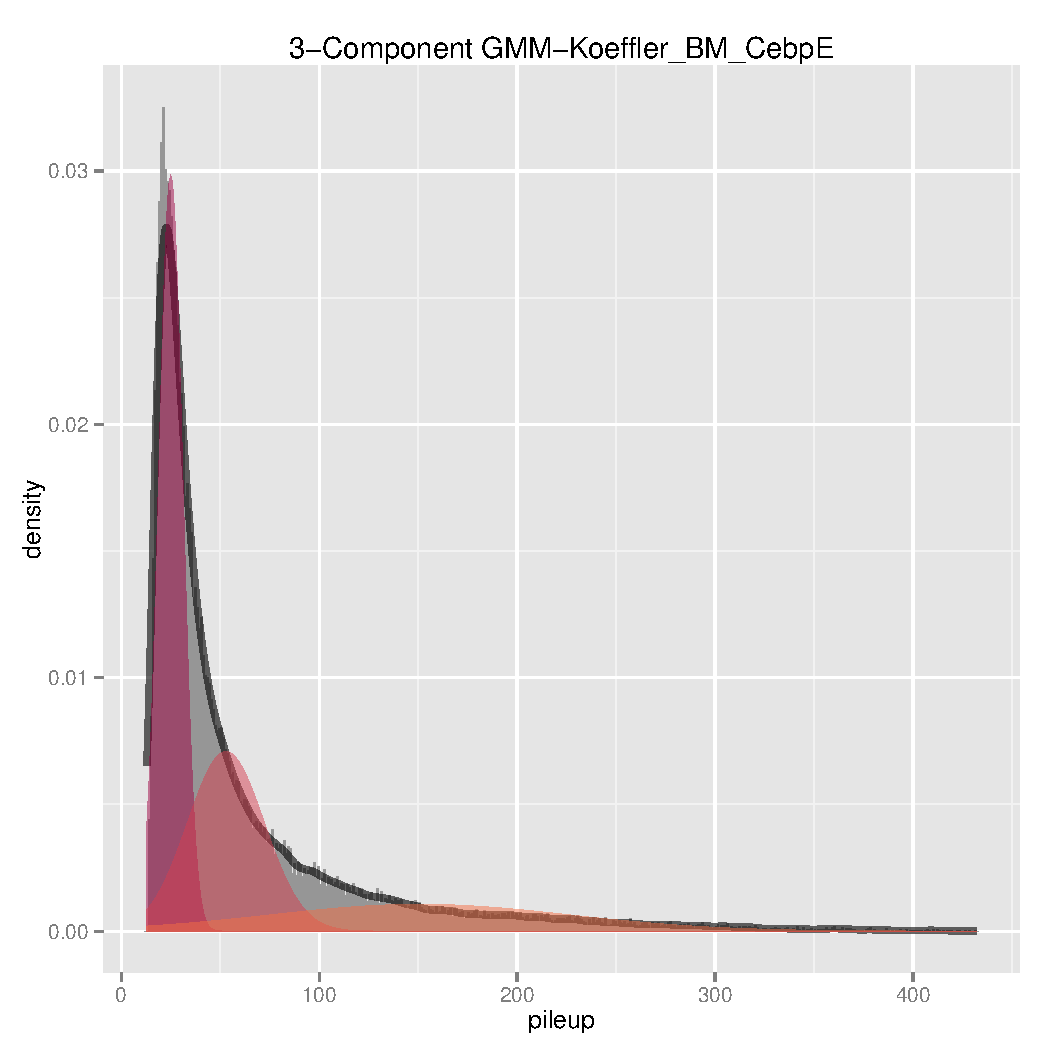
\includegraphics[width = 2in]{figs/Koeffler_BM_CebpE_GMM_ModelVisualization_comp3.pdf}}
    \subfloat{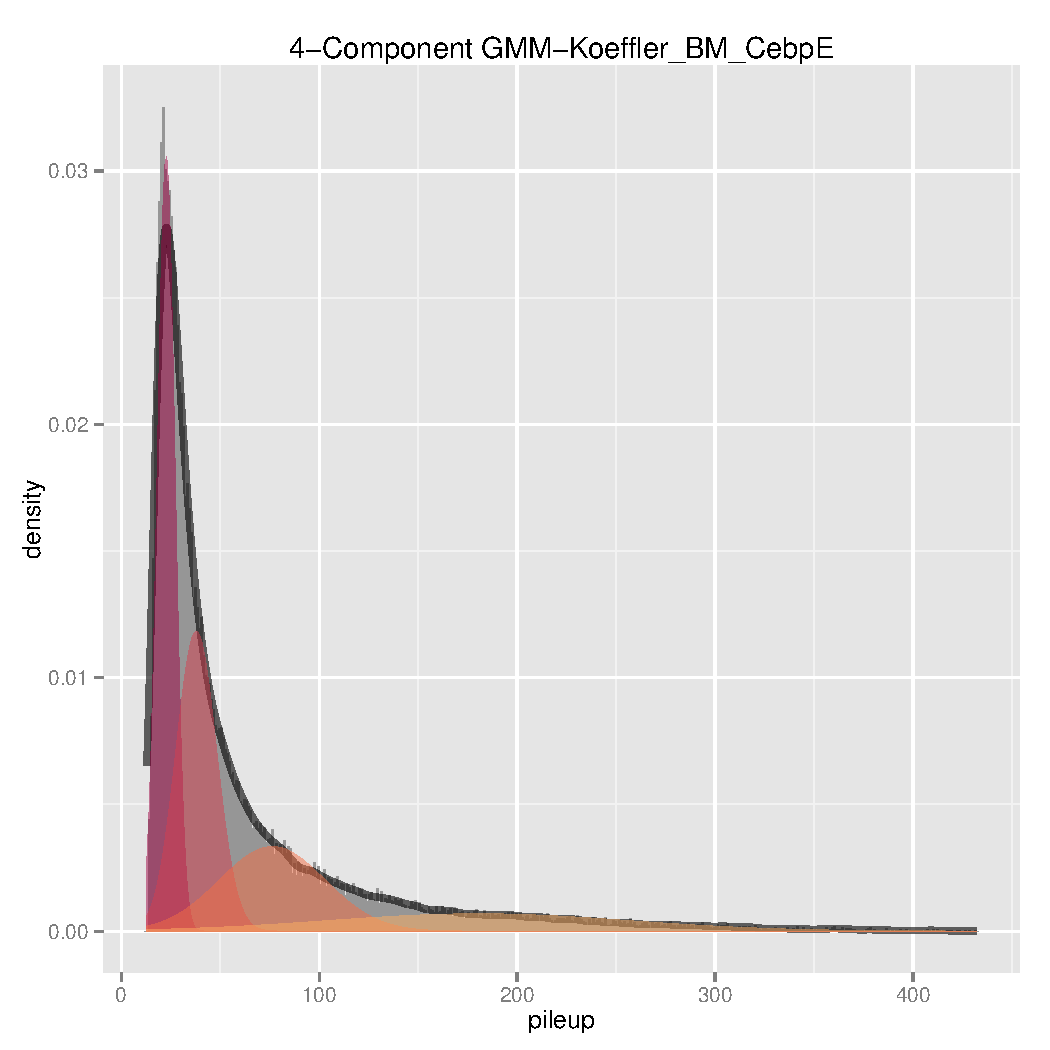
\includegraphics[width = 2in]{figs/Koeffler_BM_CebpE_GMM_ModelVisualization_comp4.pdf}}
    \\
    \subfloat{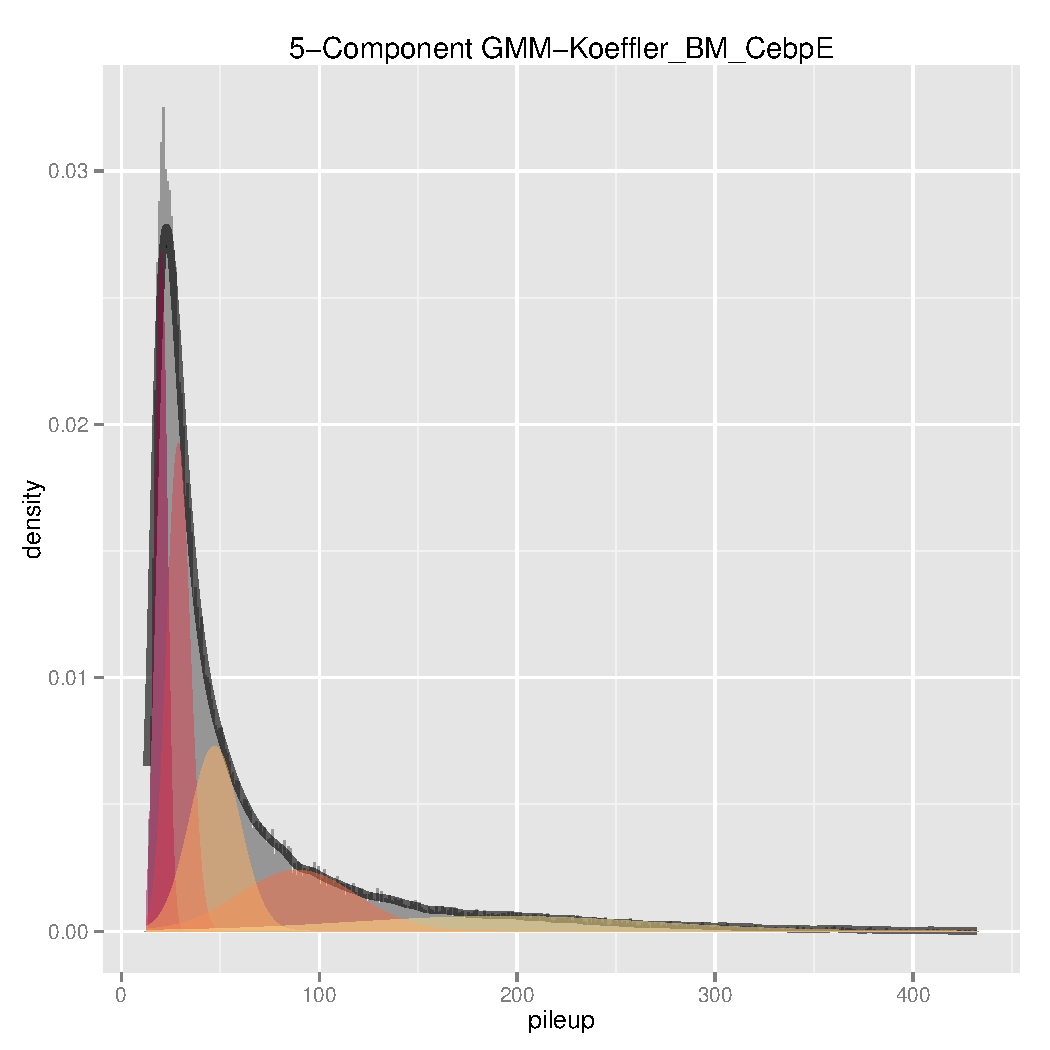
\includegraphics[width = 2in]{figs/Koeffler_BM_CebpE_GMM_ModelVisualization_comp5.pdf}}
    \subfloat{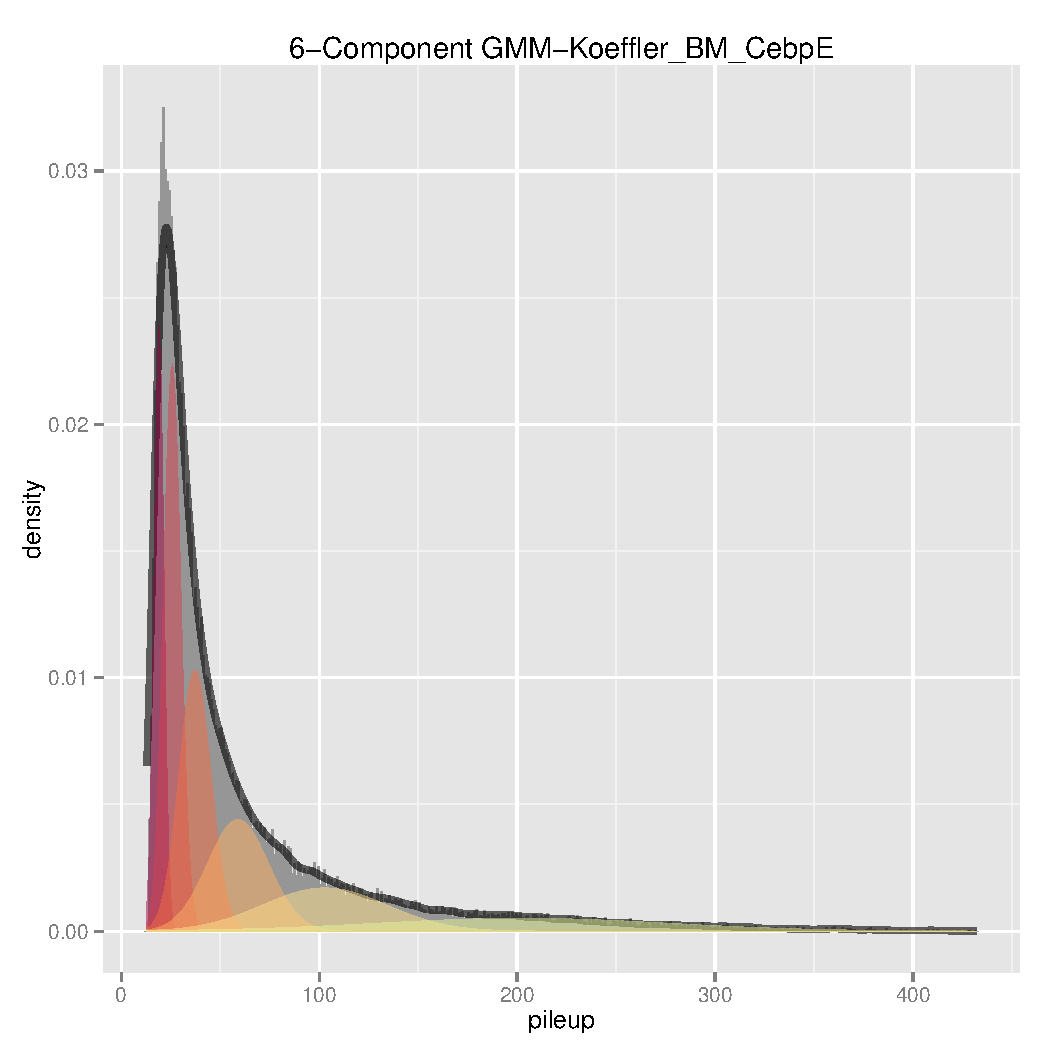
\includegraphics[width = 2in]{figs/Koeffler_BM_CebpE_GMM_ModelVisualization_comp6.pdf}}
    \subfloat{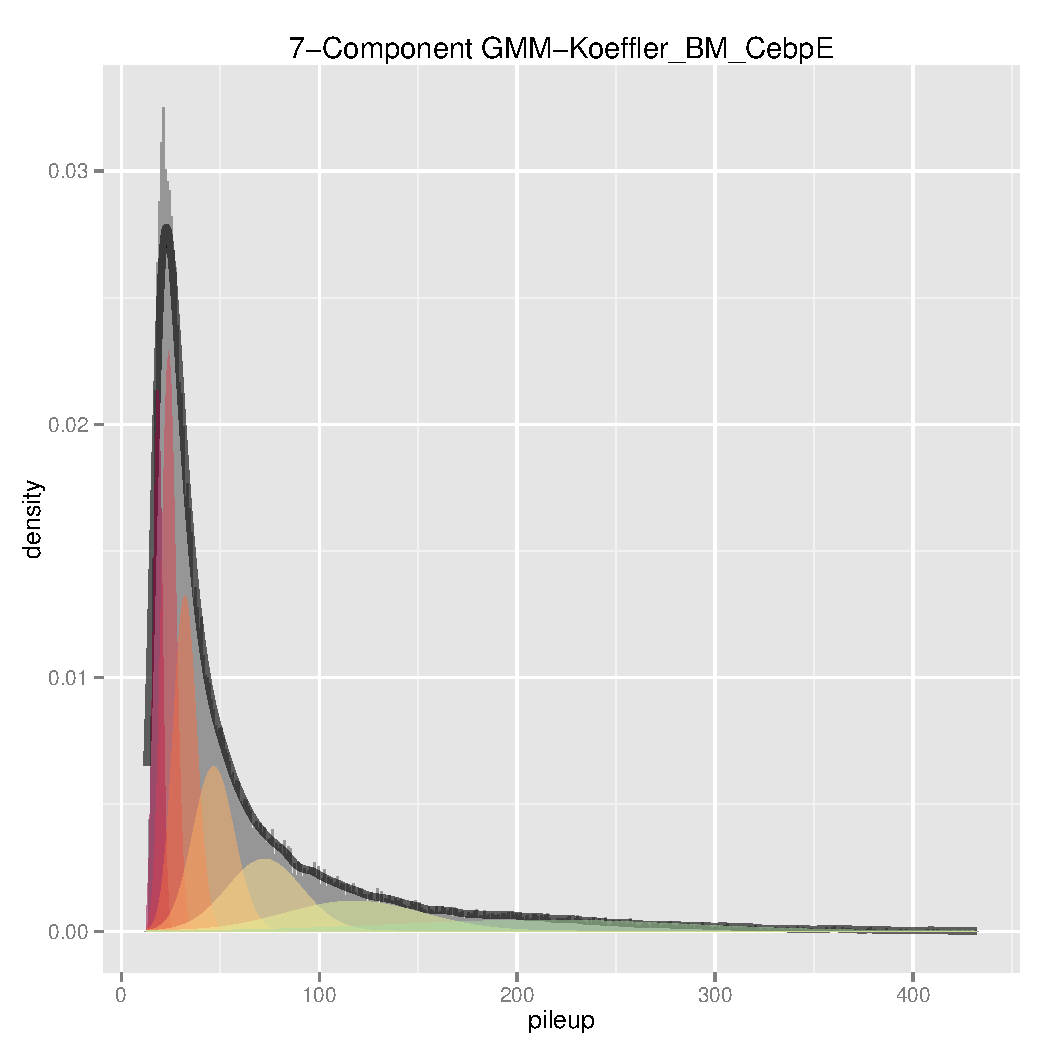
\includegraphics[width = 2in]{figs/Koeffler_BM_CebpE_GMM_ModelVisualization_comp7.pdf}}
    \\
    \subfloat{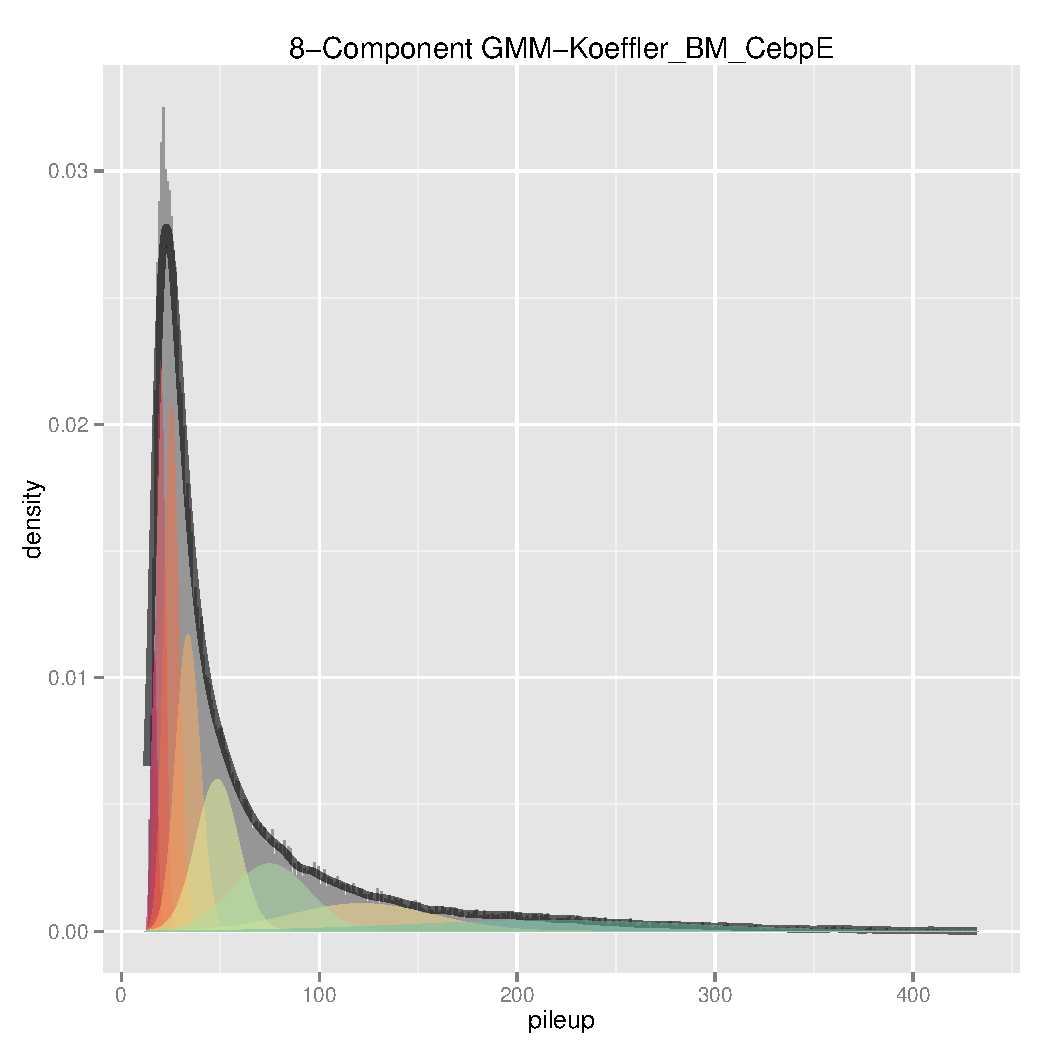
\includegraphics[width = 2in]{figs/Koeffler_BM_CebpE_GMM_ModelVisualization_comp8.pdf}}
    \subfloat{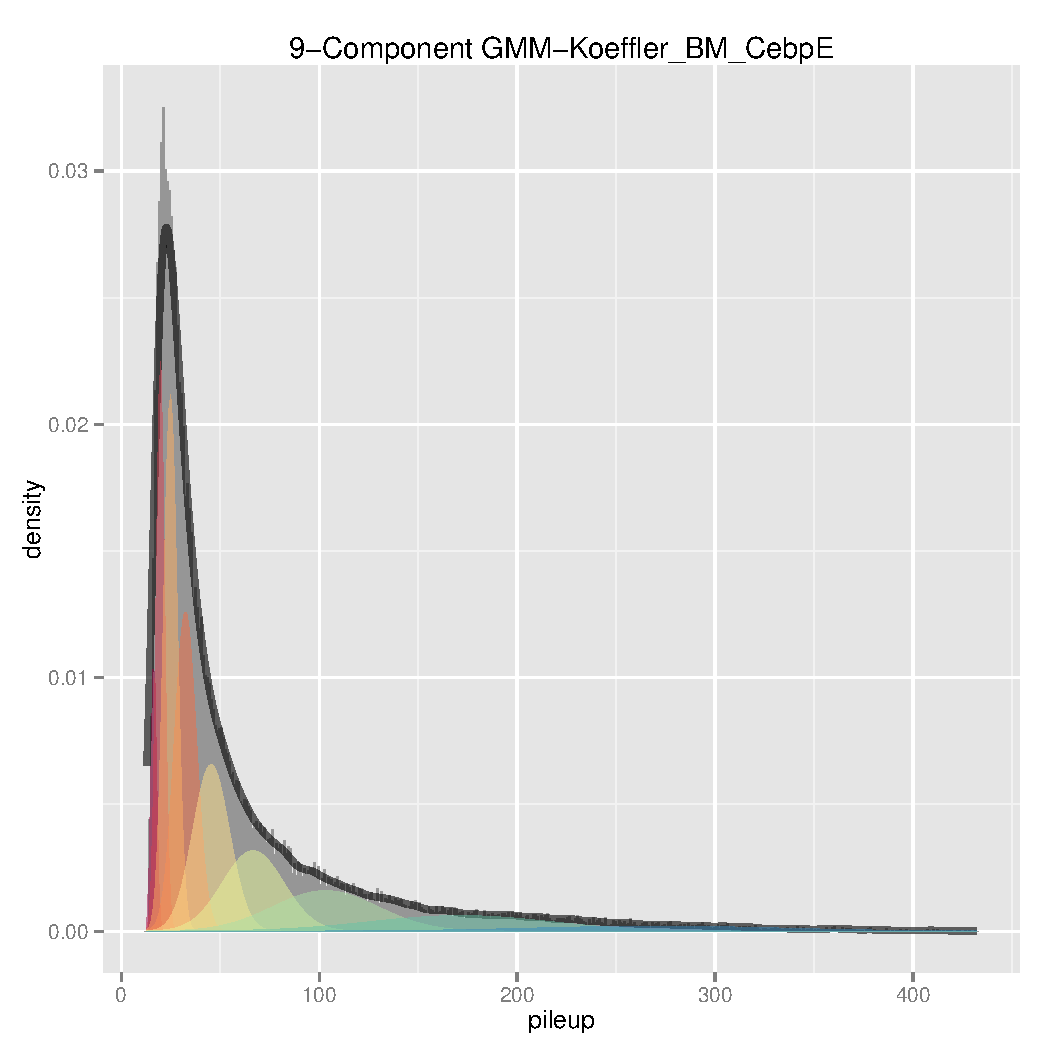
\includegraphics[width = 2in]{figs/Koeffler_BM_CebpE_GMM_ModelVisualization_comp9.pdf}}
    \subfloat{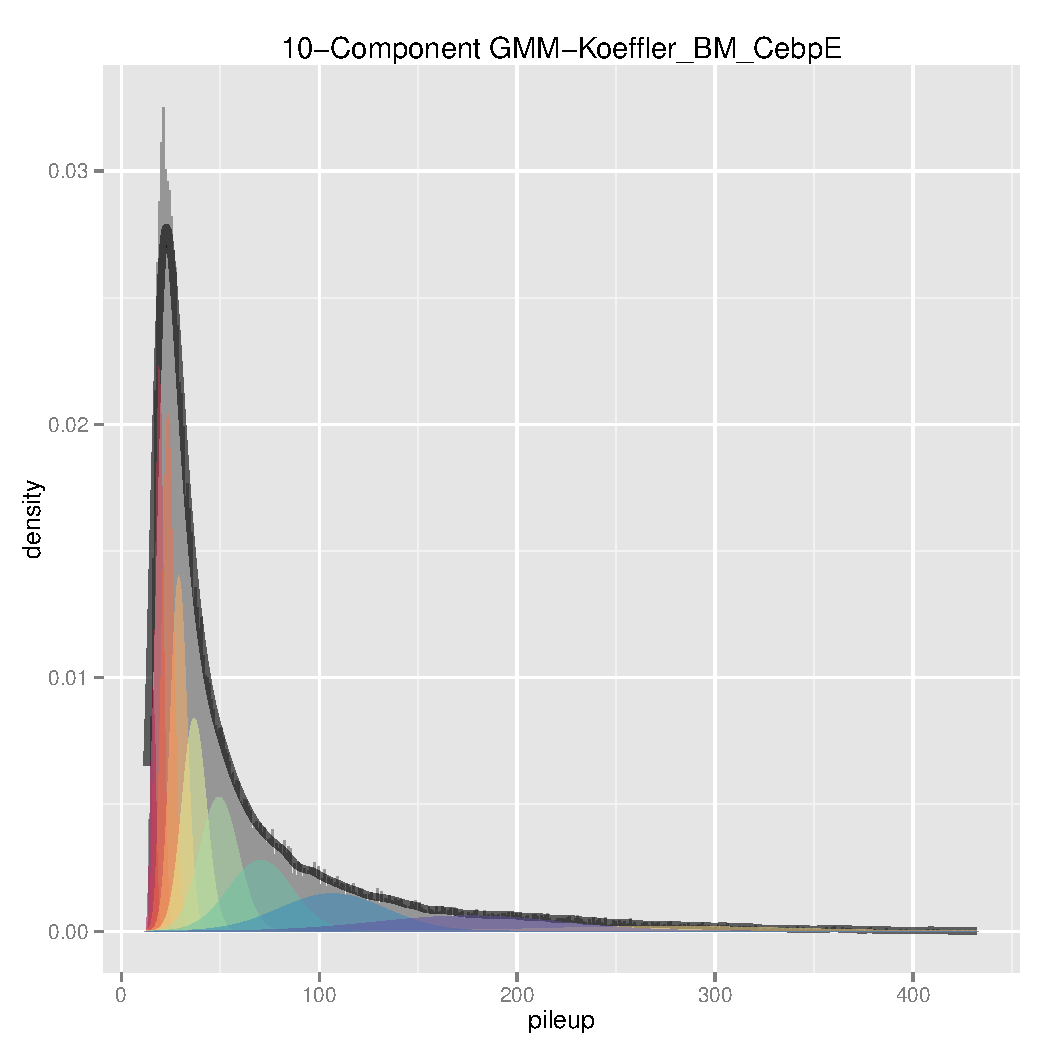
\includegraphics[width = 2in]{figs/Koeffler_BM_CebpE_GMM_ModelVisualization_comp10.pdf}}
    \caption{ChIPseq Peaks Fit with GMMs Ranging from Two to Ten Components}
    \label{fig:FittingChIPGMM}
\end{figure}
\clearpage

\subsection{Fitted NBMs Visualized on ChiP-seq distributions}

\begin{knitrout}
\definecolor{shadecolor}{rgb}{0.969, 0.969, 0.969}\color{fgcolor}\begin{kframe}
\begin{alltt}
\hlkwd{visualizeFitMMs}\hlstd{(}\hlkwc{X}\hlstd{=Koeffler_BM_CebpE,} \hlkwc{MMs_list}\hlstd{=NBMs_list_Koeffler_BM_CebpE,}
                \hlkwc{max_k}\hlstd{=}\hlnum{10}\hlstd{,} \hlkwc{output_n}\hlstd{=}\hlstr{'figs/Koeffler_BM_CebpE_NBM_ModelVisualization'}\hlstd{,}
                \hlkwc{model} \hlstd{=} \hlstr{'NBM'}\hlstd{,} \hlkwc{titleName}\hlstd{=}\hlstr{'Koeffler_BM_CebpE'}\hlstd{)}
\end{alltt}
\end{kframe}
\end{knitrout}

\begin{figure}[!htp]
    \centering
    \subfloat{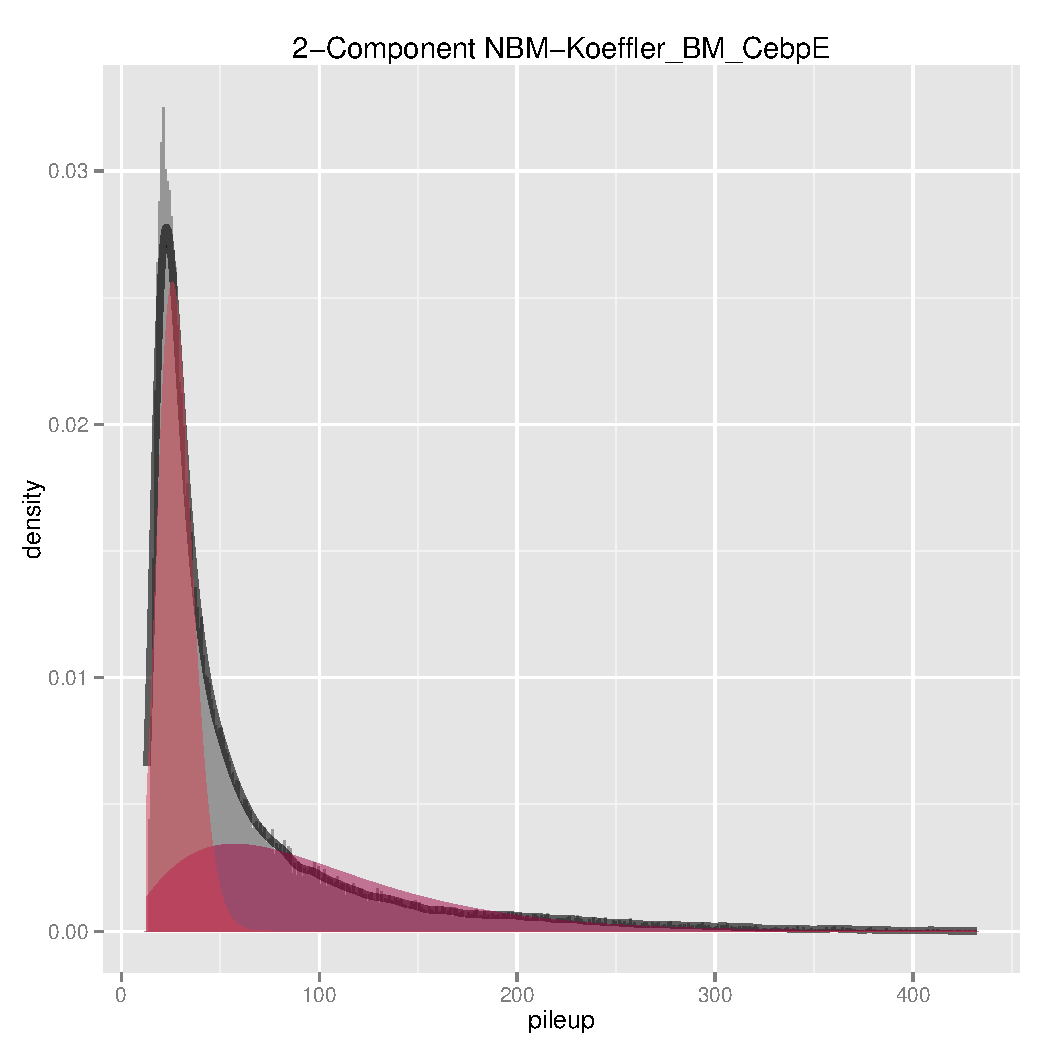
\includegraphics[width = 2in]{figs/Koeffler_BM_CebpE_NBM_ModelVisualization_comp2.pdf}}
    \subfloat{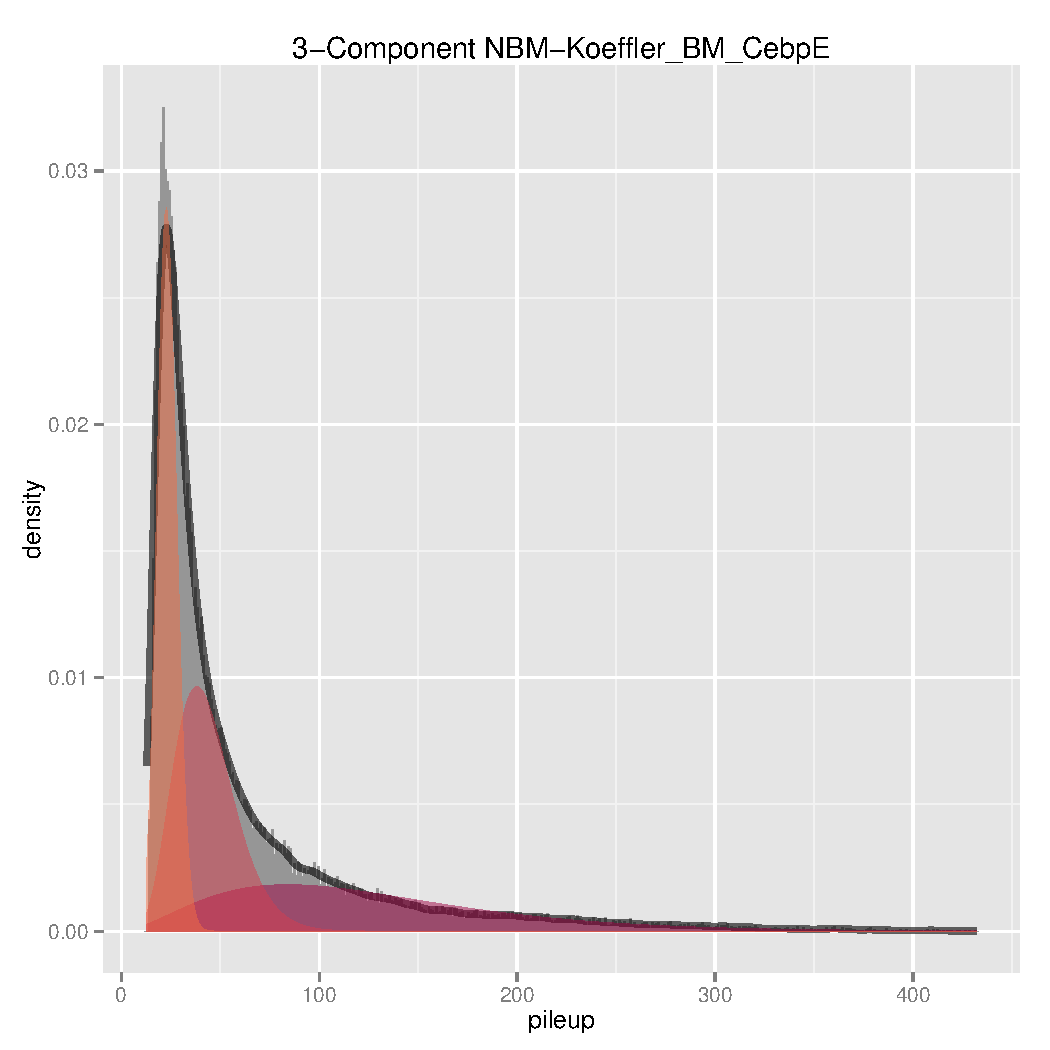
\includegraphics[width = 2in]{figs/Koeffler_BM_CebpE_NBM_ModelVisualization_comp3.pdf}}
    \subfloat{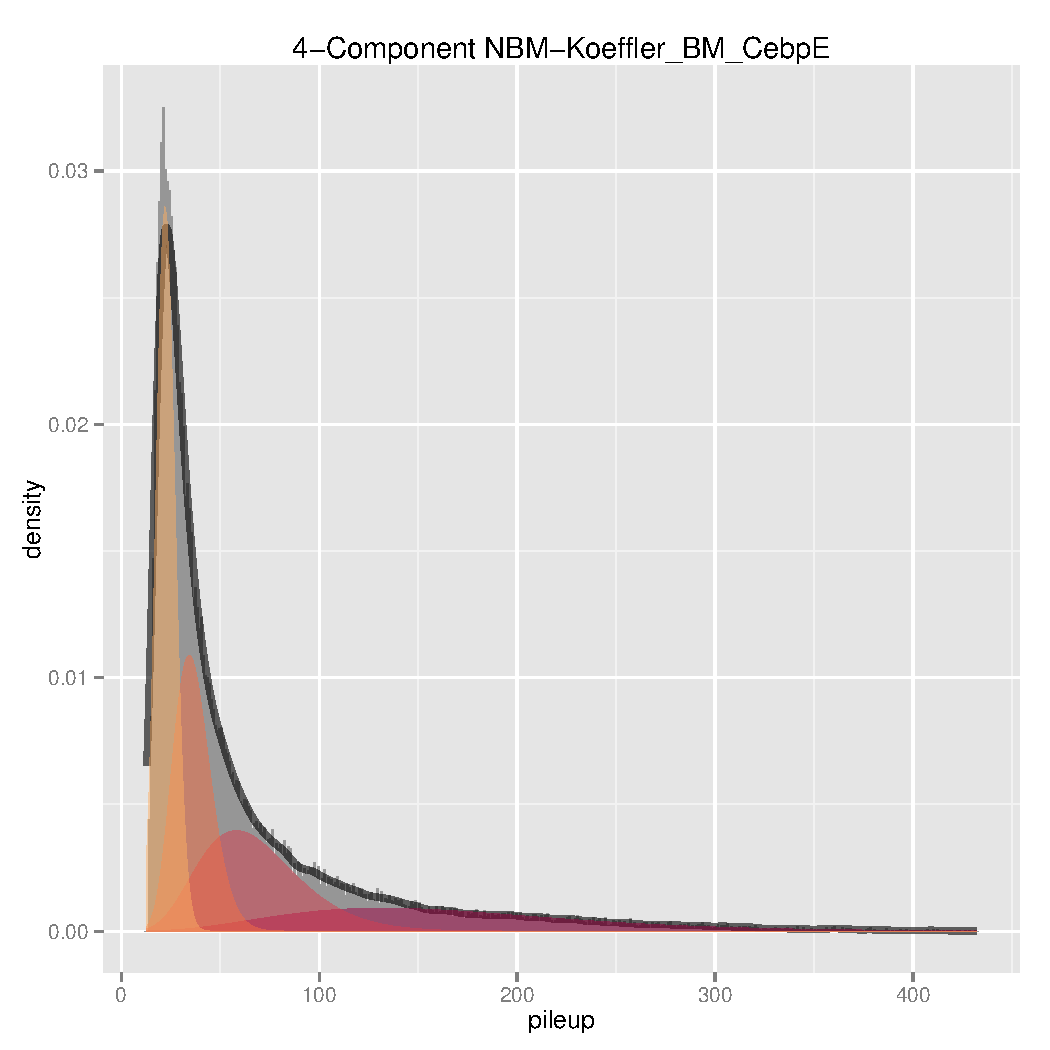
\includegraphics[width = 2in]{figs/Koeffler_BM_CebpE_NBM_ModelVisualization_comp4.pdf}}
    \\
    \subfloat{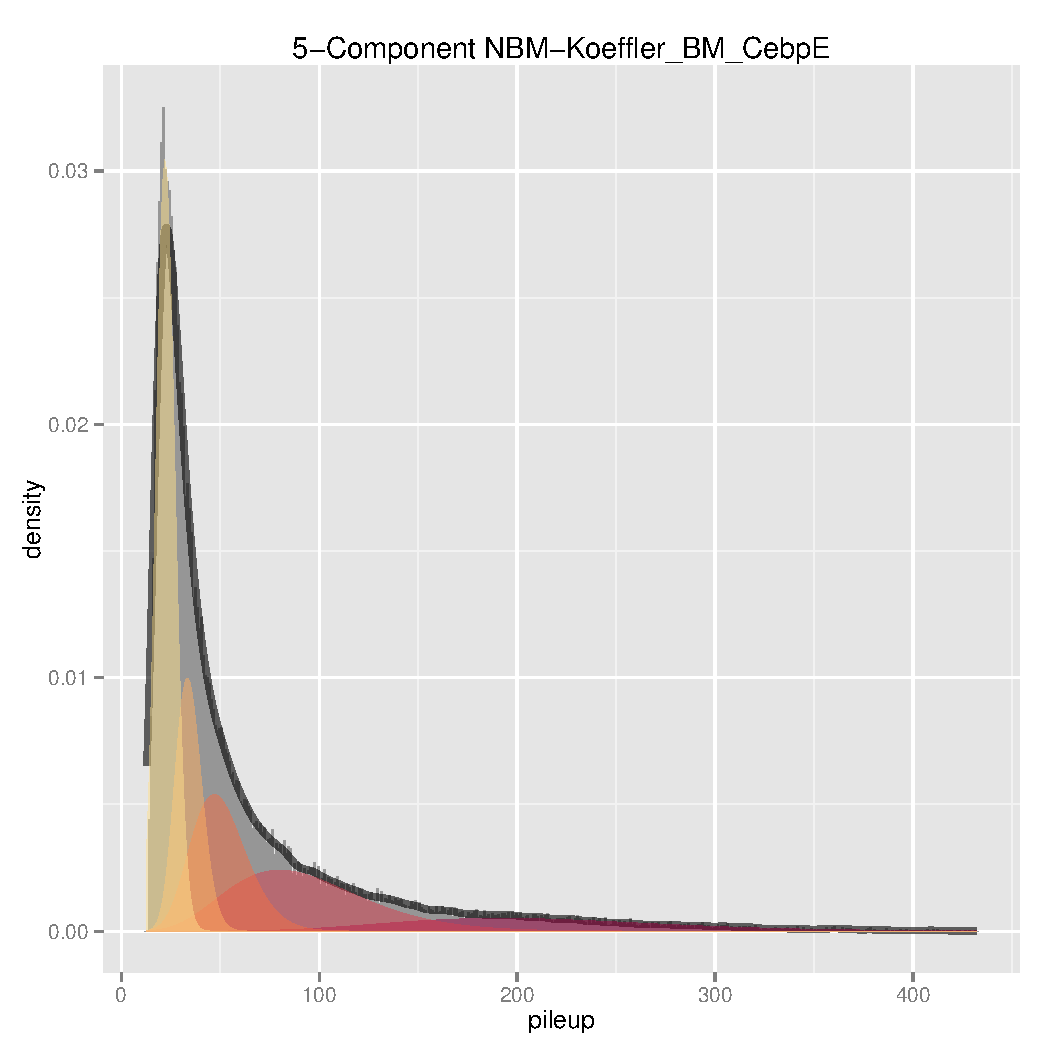
\includegraphics[width = 2in]{figs/Koeffler_BM_CebpE_NBM_ModelVisualization_comp5.pdf}}
    \subfloat{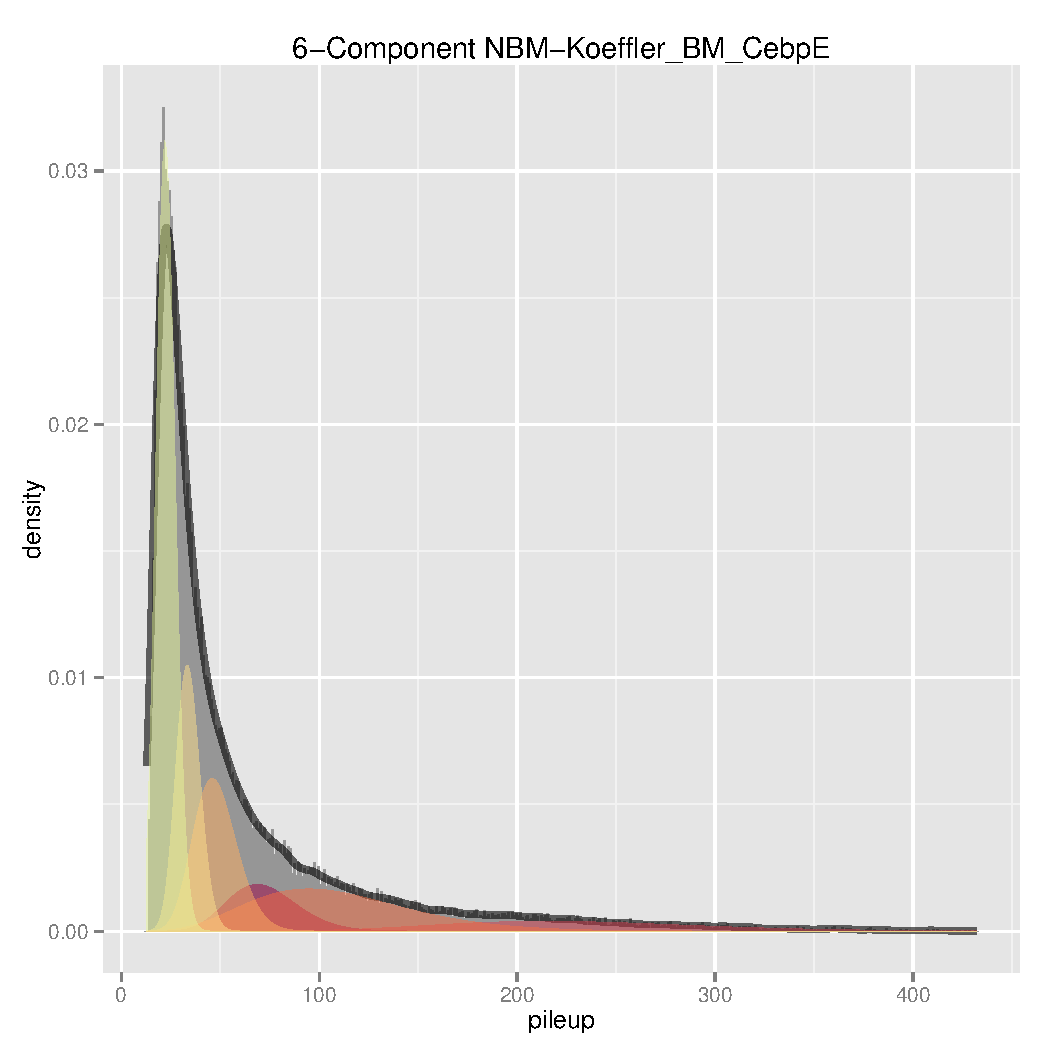
\includegraphics[width = 2in]{figs/Koeffler_BM_CebpE_NBM_ModelVisualization_comp6.pdf}}
    \subfloat{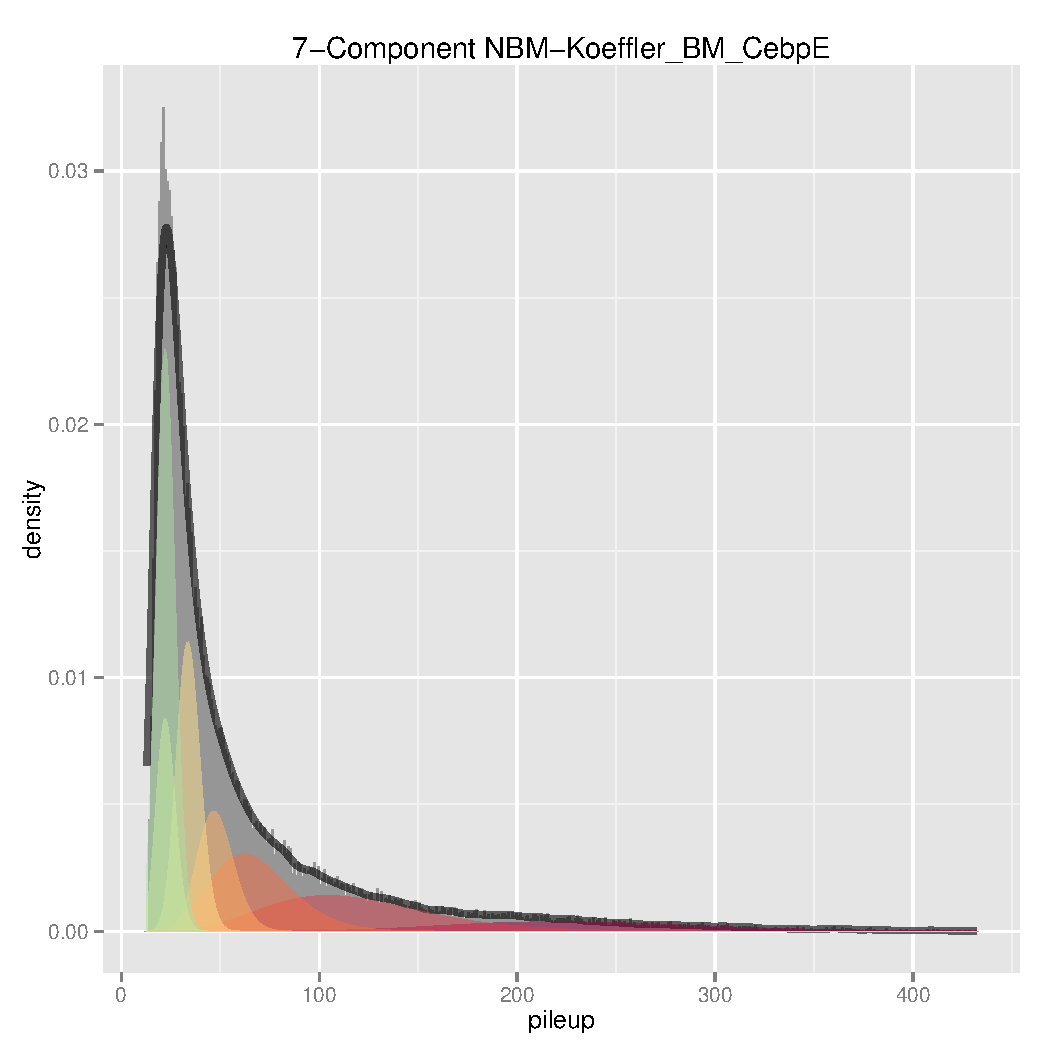
\includegraphics[width = 2in]{figs/Koeffler_BM_CebpE_NBM_ModelVisualization_comp7.pdf}}
    \\
    \subfloat{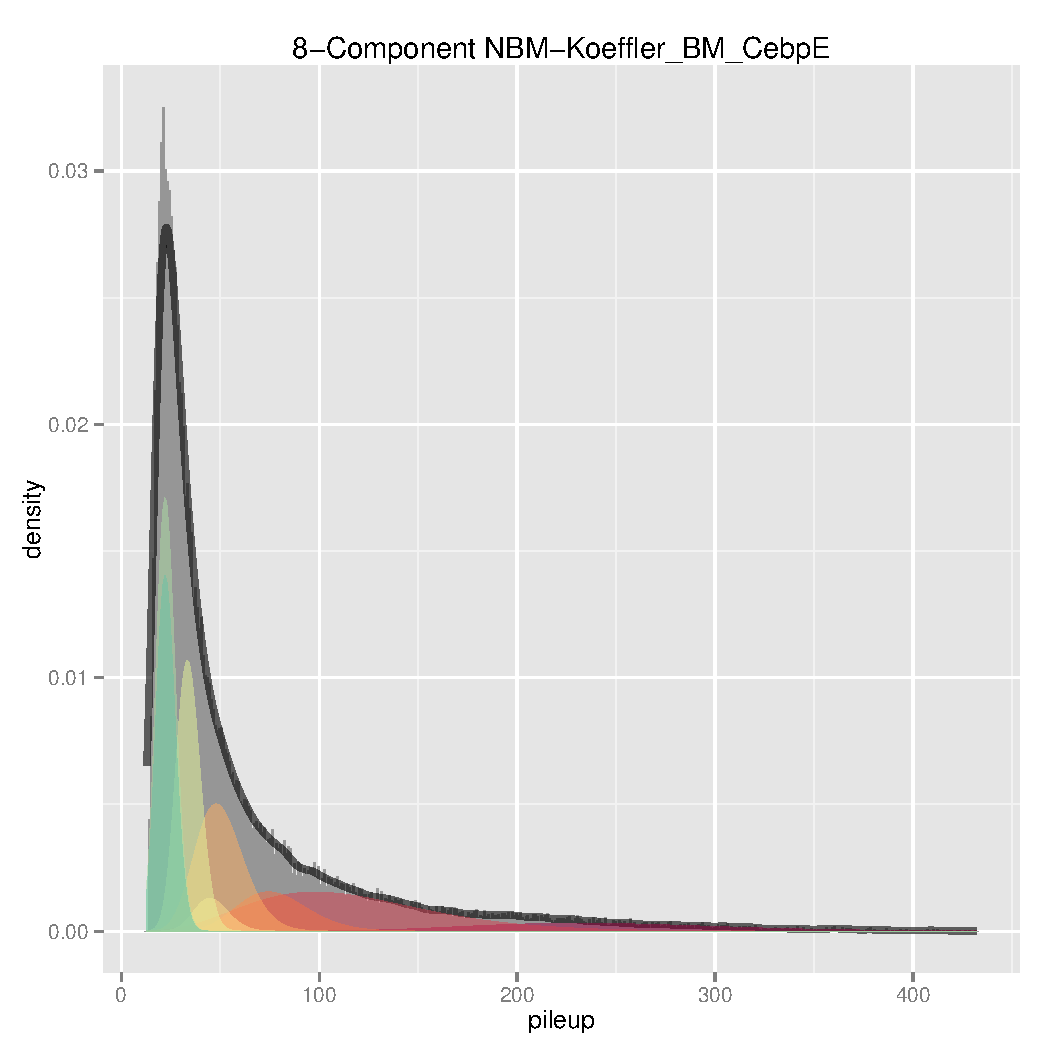
\includegraphics[width = 2in]{figs/Koeffler_BM_CebpE_NBM_ModelVisualization_comp8.pdf}}
    \subfloat{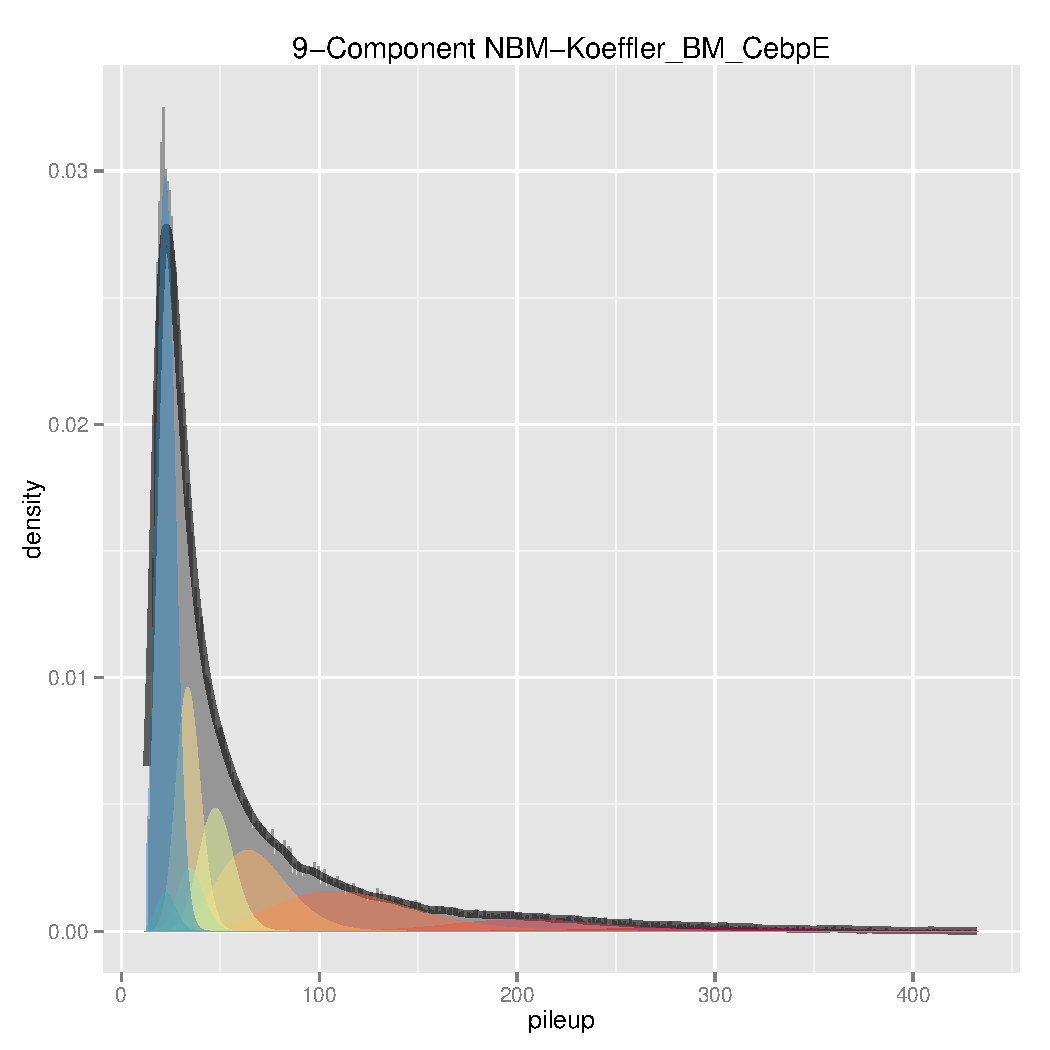
\includegraphics[width = 2in]{figs/Koeffler_BM_CebpE_NBM_ModelVisualization_comp9.pdf}}
    \subfloat{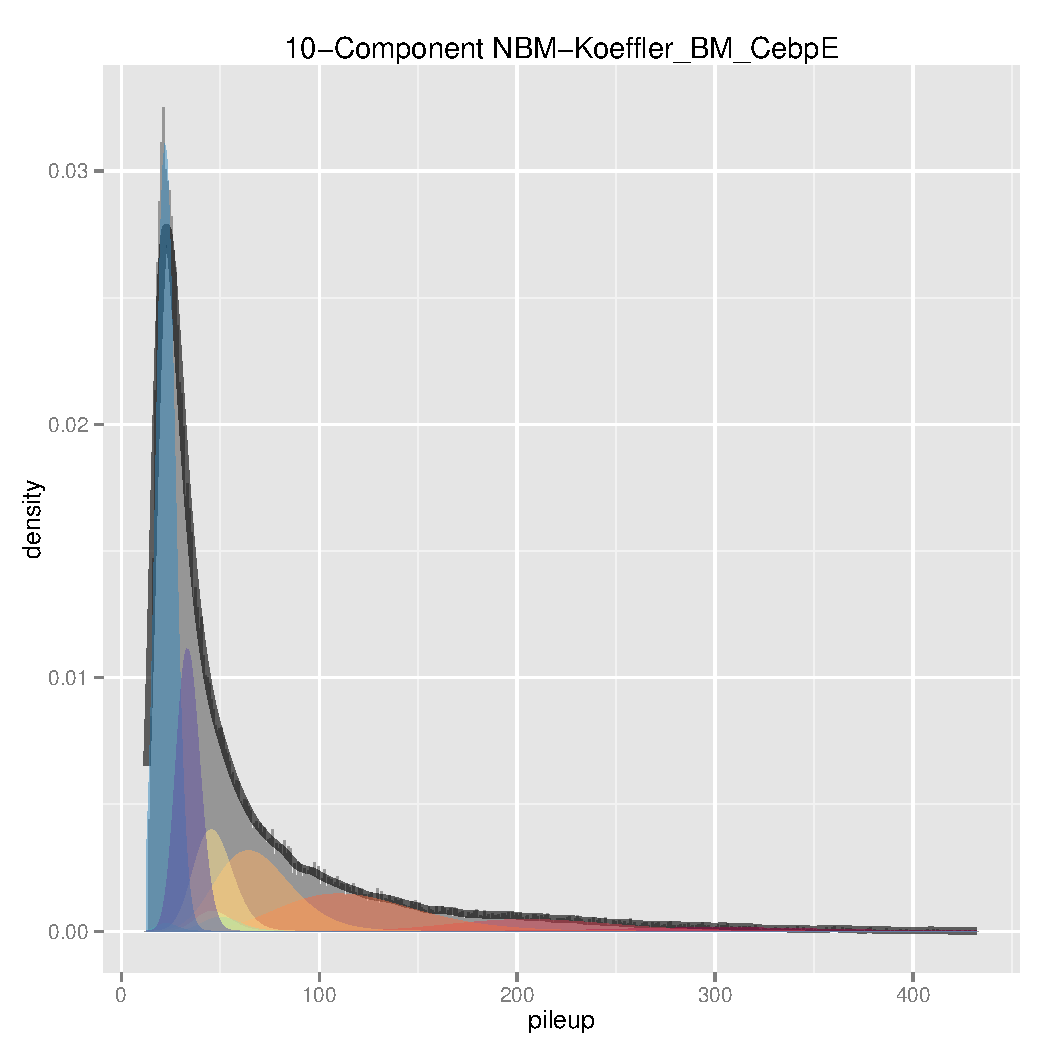
\includegraphics[width = 2in]{figs/Koeffler_BM_CebpE_NBM_ModelVisualization_comp10.pdf}}
    \caption{ChIPseq Peaks Fit with NBMs Ranging from Two to Ten Components}
    \label{fig:FittingChIPNBM}
\end{figure}
\clearpage

\section{Emperical vs Estimate Distribution}
Here, we assess for the possible overfit of our fitting mixture models by comparing the emperical and overal estimate distribution from the mixture models.

\subsection{Comparing Density Estimates: Empirical vs Gaussian Mixture (GMM)}
\begin{figure}[!htp]
    \centering
    \subfloat{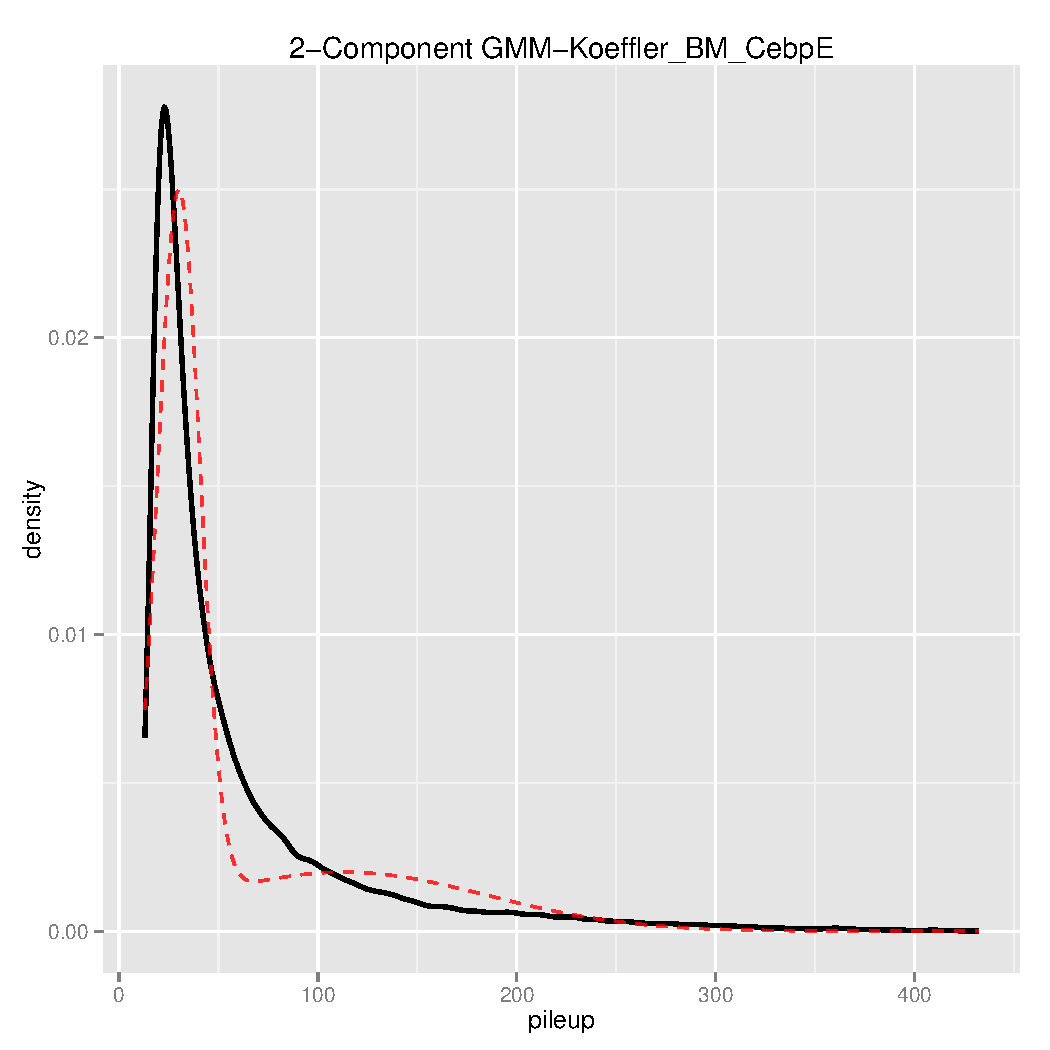
\includegraphics[width = 2in]{figs/Koeffler_BM_CebpE_GMM_ModelVisualization_comp2_empVsModel.pdf}}
    \subfloat{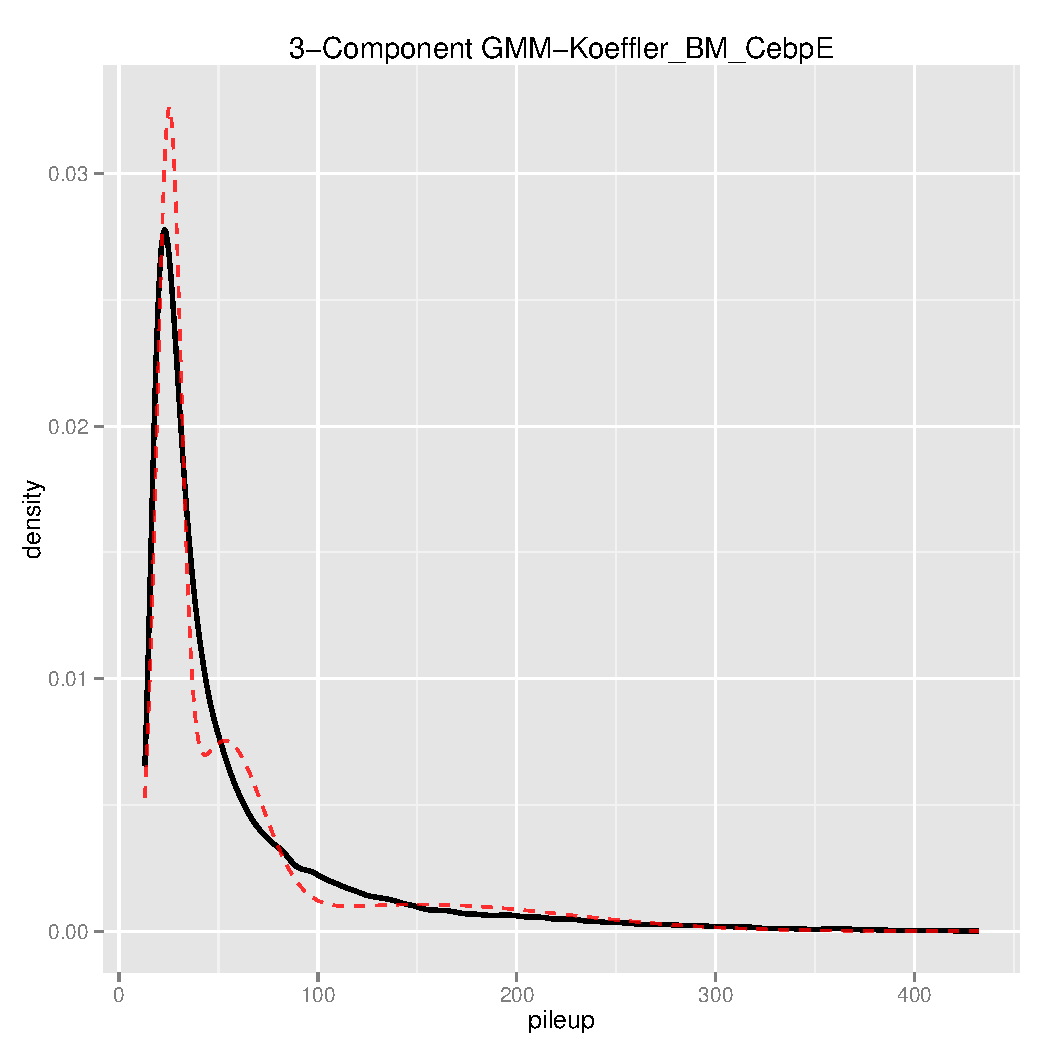
\includegraphics[width = 2in]{figs/Koeffler_BM_CebpE_GMM_ModelVisualization_comp3_empVsModel.pdf}}
    \subfloat{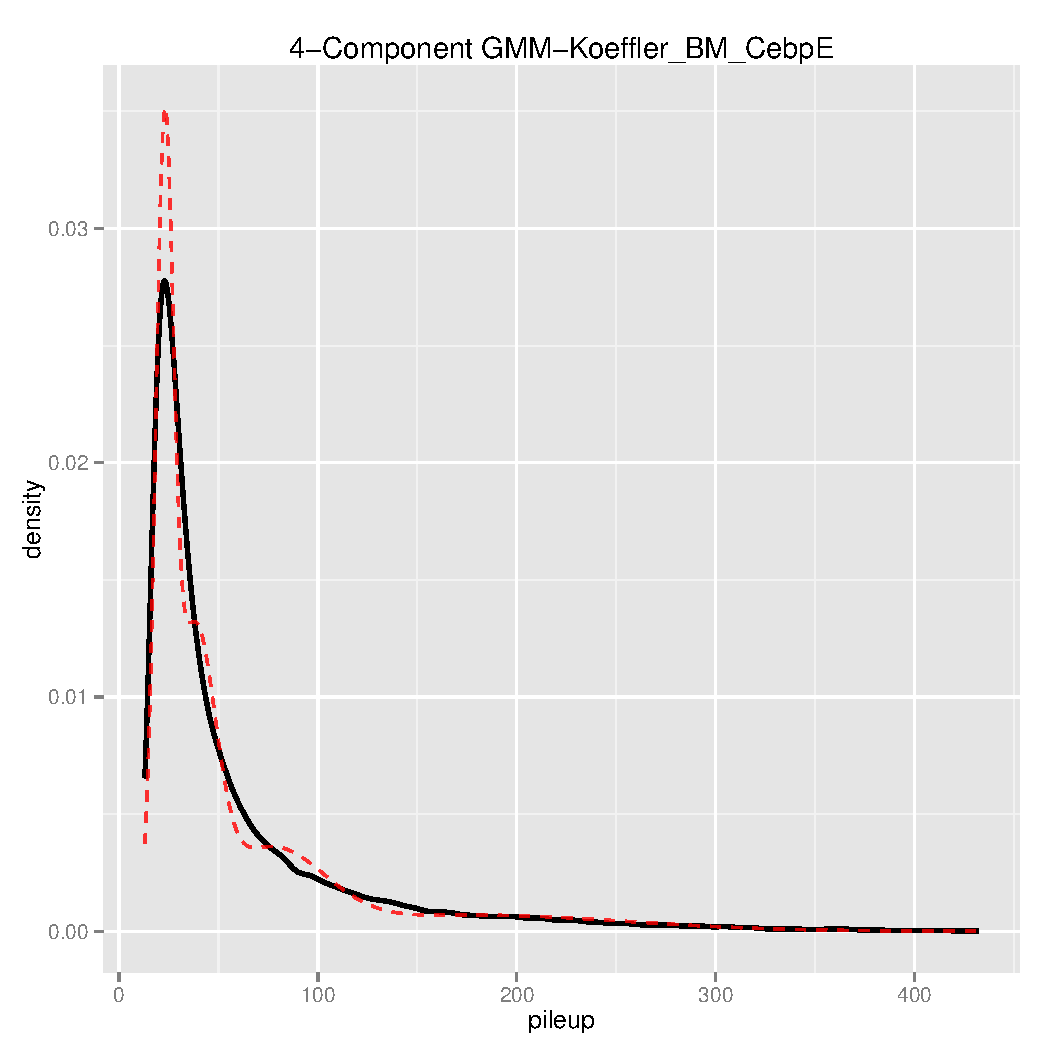
\includegraphics[width = 2in]{figs/Koeffler_BM_CebpE_GMM_ModelVisualization_comp4_empVsModel.pdf}}
    \\
    \subfloat{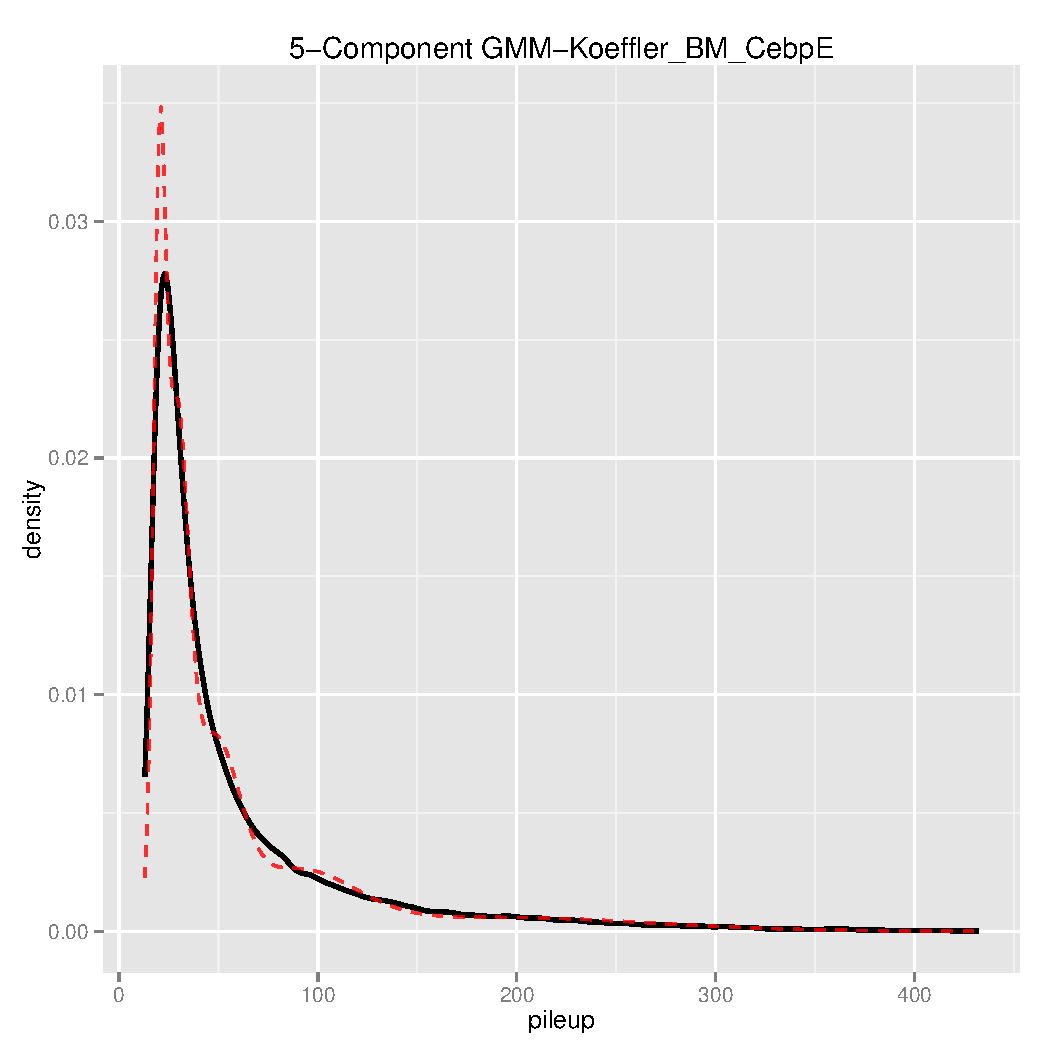
\includegraphics[width = 2in]{figs/Koeffler_BM_CebpE_GMM_ModelVisualization_comp5_empVsModel.pdf}}
    \subfloat{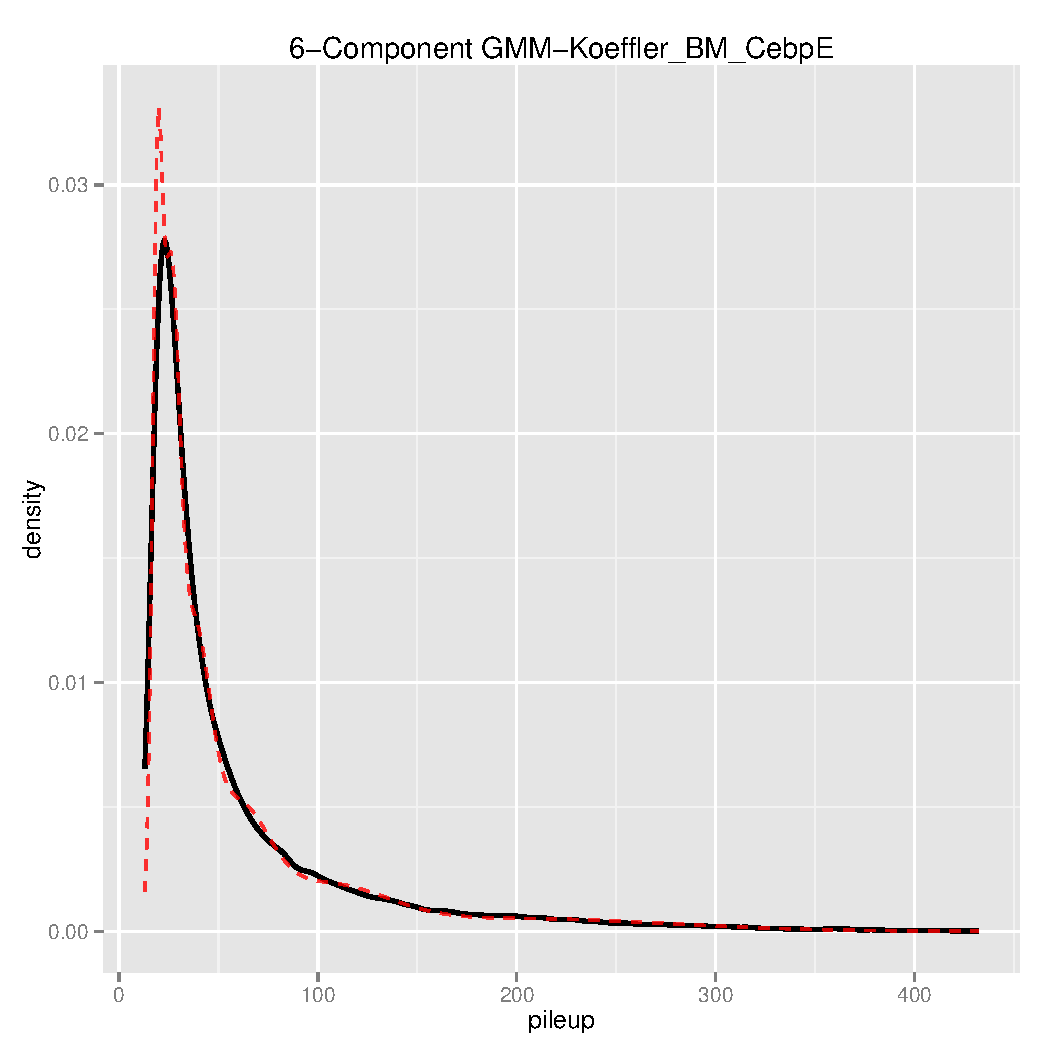
\includegraphics[width = 2in]{figs/Koeffler_BM_CebpE_GMM_ModelVisualization_comp6_empVsModel.pdf}}
    \subfloat{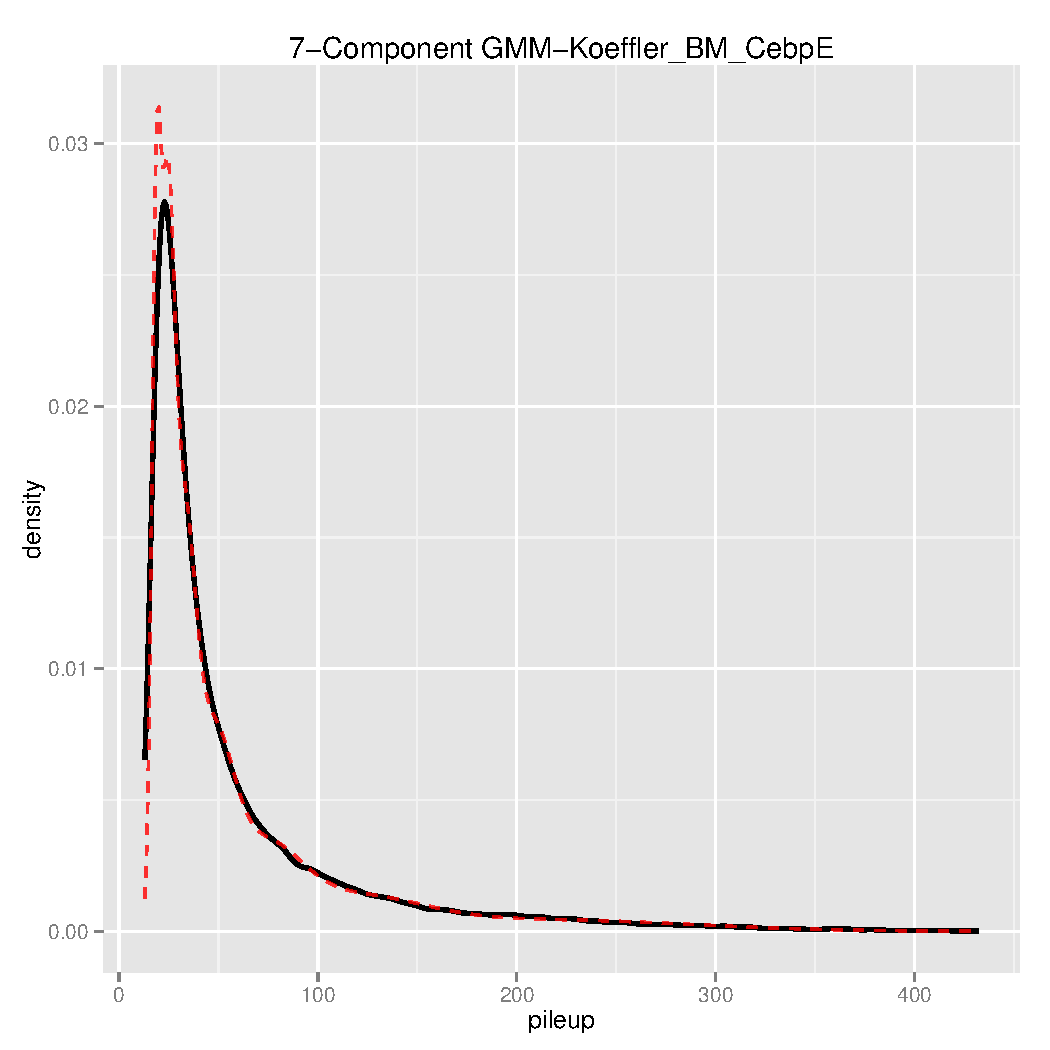
\includegraphics[width = 2in]{figs/Koeffler_BM_CebpE_GMM_ModelVisualization_comp7_empVsModel.pdf}}
    \\
    \subfloat{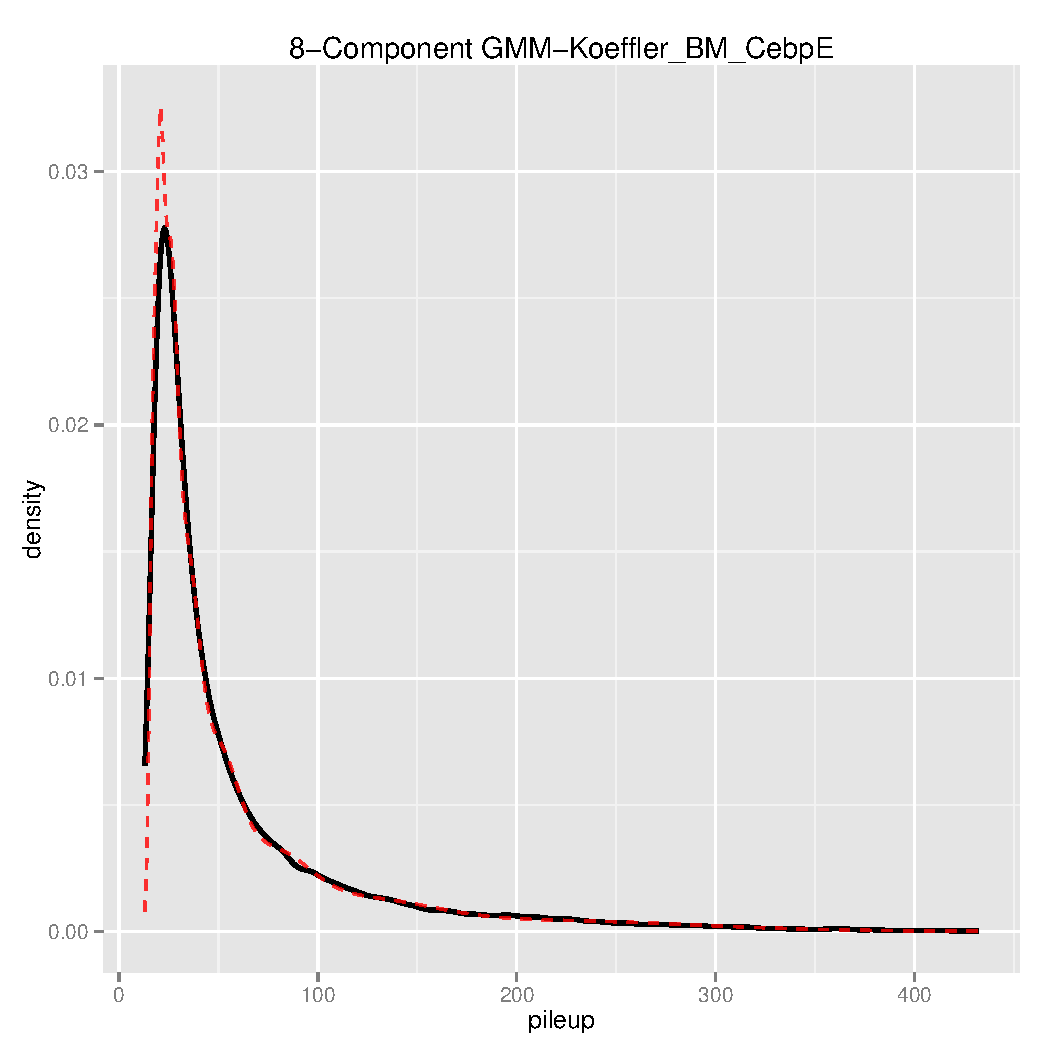
\includegraphics[width = 2in]{figs/Koeffler_BM_CebpE_GMM_ModelVisualization_comp8_empVsModel.pdf}}
    \subfloat{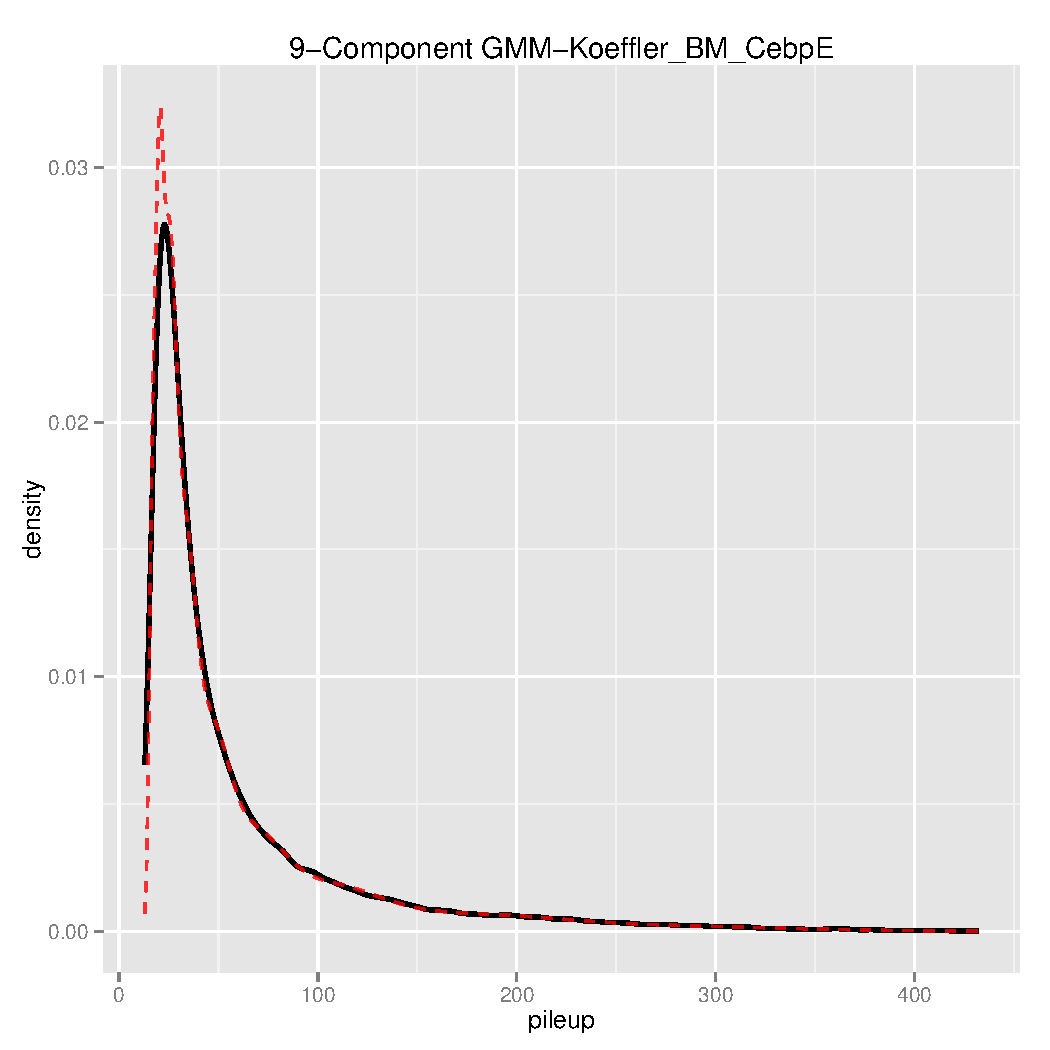
\includegraphics[width = 2in]{figs/Koeffler_BM_CebpE_GMM_ModelVisualization_comp9_empVsModel.pdf}}
    \subfloat{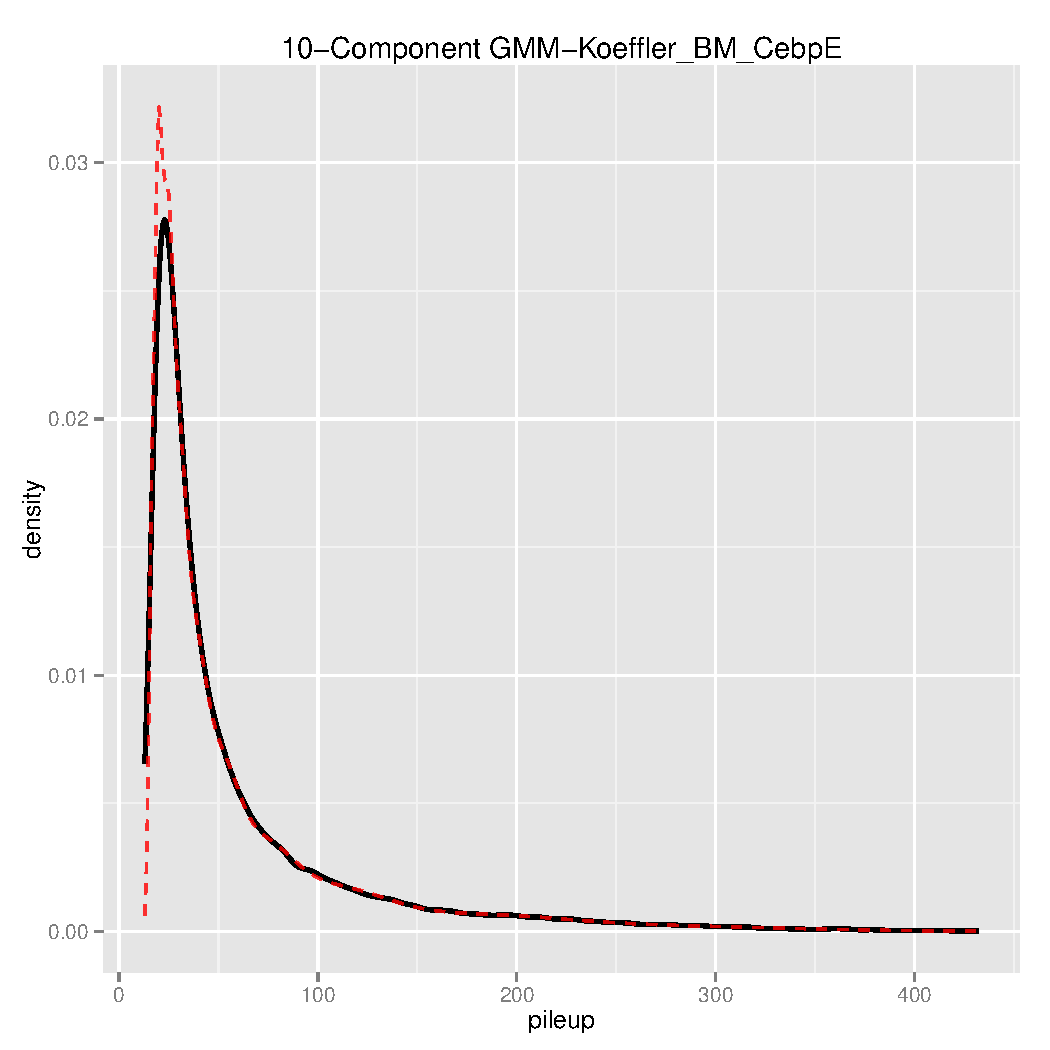
\includegraphics[width = 2in]{figs/Koeffler_BM_CebpE_GMM_ModelVisualization_comp10_empVsModel.pdf}}
    \caption{Comparing Density Estimates: Empirical Vs Gaussian Mixture. Empirical and gaussian density are coloured with black and dashed-red, respectively.}
    \label{fig:empVsgauss}
\end{figure}
\clearpage

\subsection{Comparing Density Estimates: Empirical vs Gaussian Mixture (NBM)}
\begin{figure}[!htp]
    \centering
    \subfloat{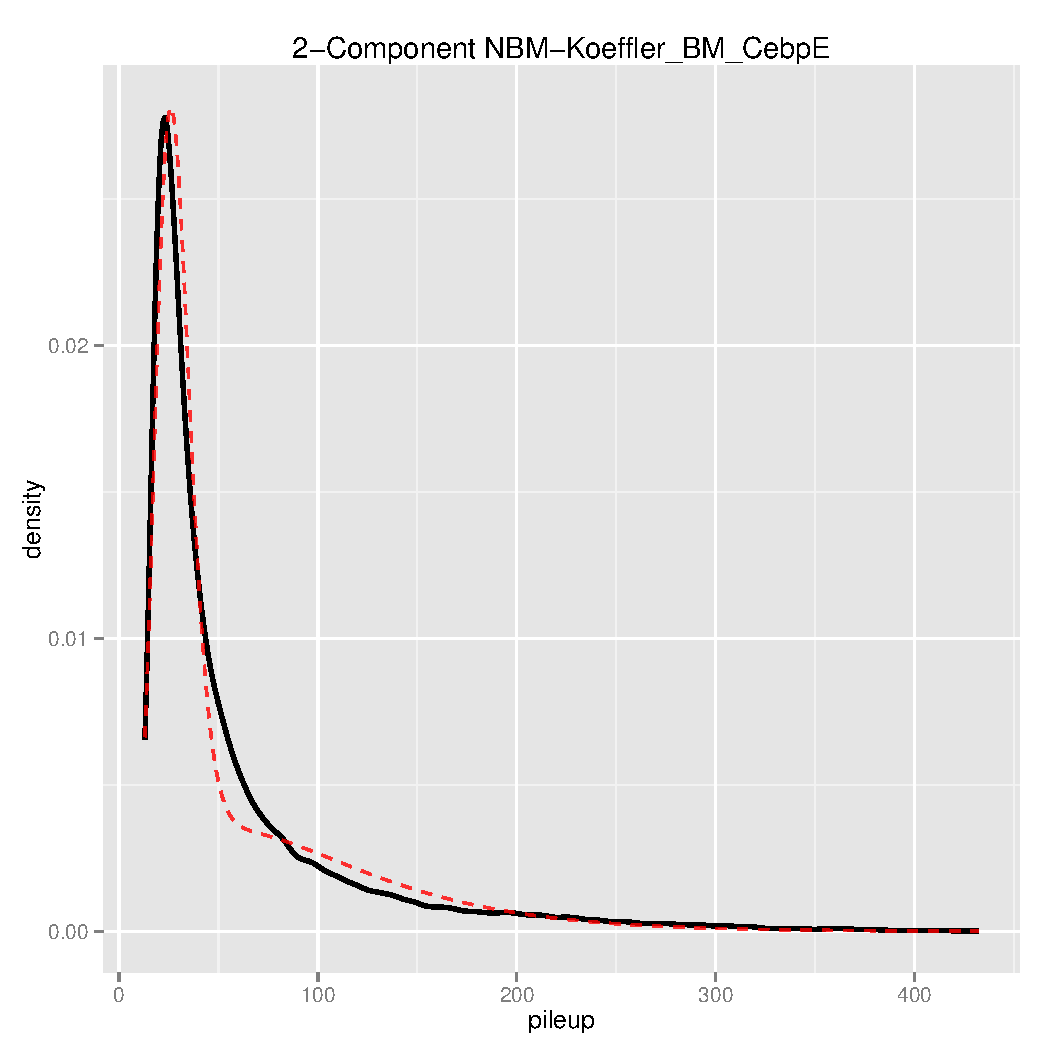
\includegraphics[width = 2in]{figs/Koeffler_BM_CebpE_NBM_ModelVisualization_comp2_empVsModel.pdf}}
    \subfloat{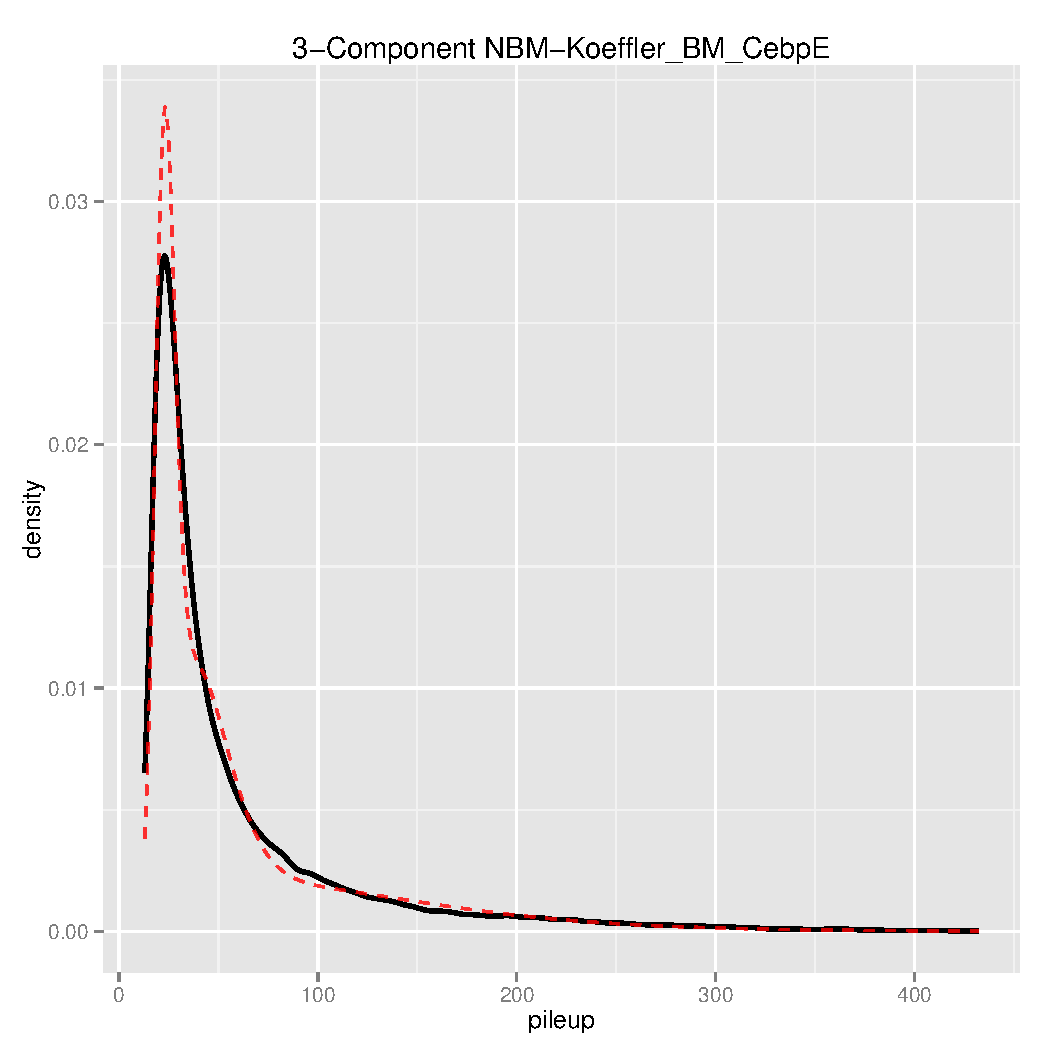
\includegraphics[width = 2in]{figs/Koeffler_BM_CebpE_NBM_ModelVisualization_comp3_empVsModel.pdf}}
    \subfloat{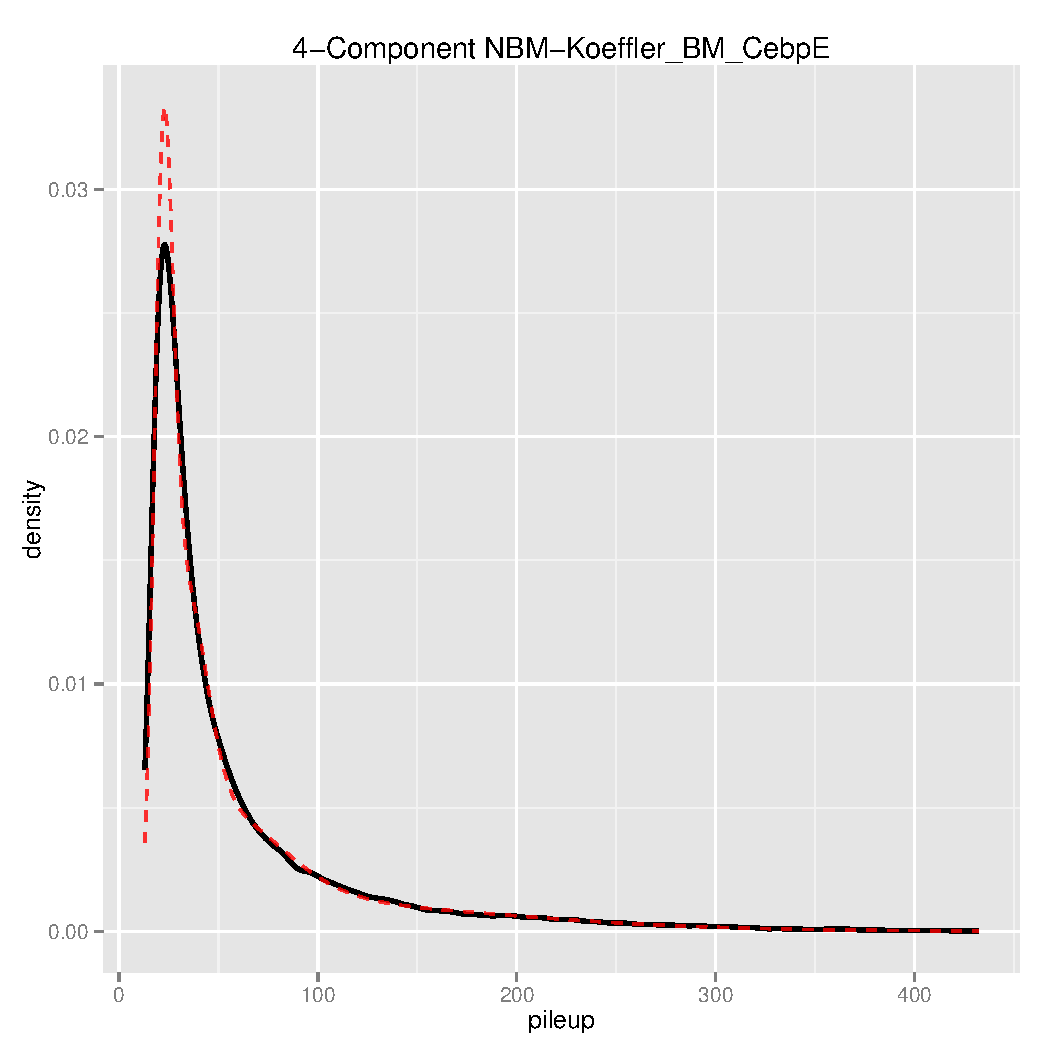
\includegraphics[width = 2in]{figs/Koeffler_BM_CebpE_NBM_ModelVisualization_comp4_empVsModel.pdf}}
    \\
    \subfloat{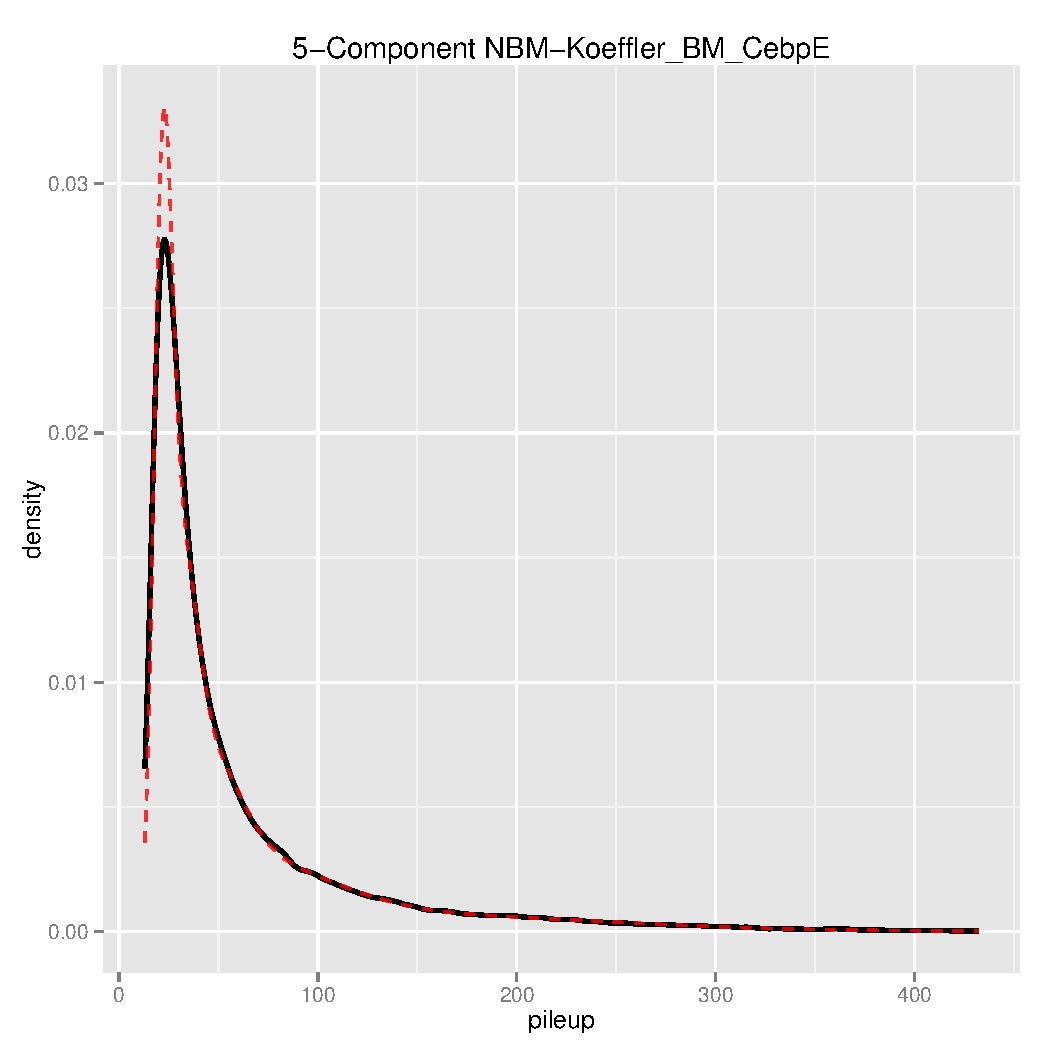
\includegraphics[width = 2in]{figs/Koeffler_BM_CebpE_NBM_ModelVisualization_comp5_empVsModel.pdf}}
    \subfloat{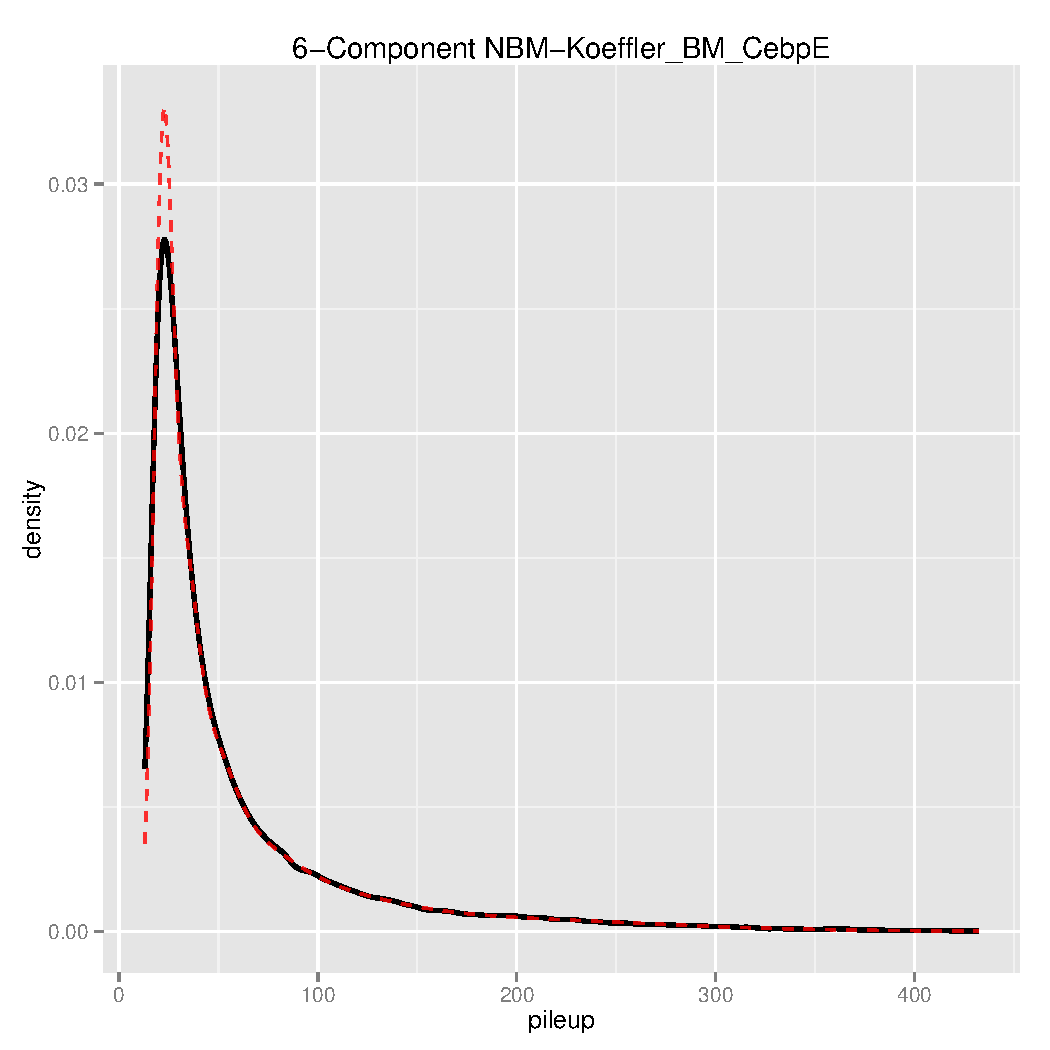
\includegraphics[width = 2in]{figs/Koeffler_BM_CebpE_NBM_ModelVisualization_comp6_empVsModel.pdf}}
    \subfloat{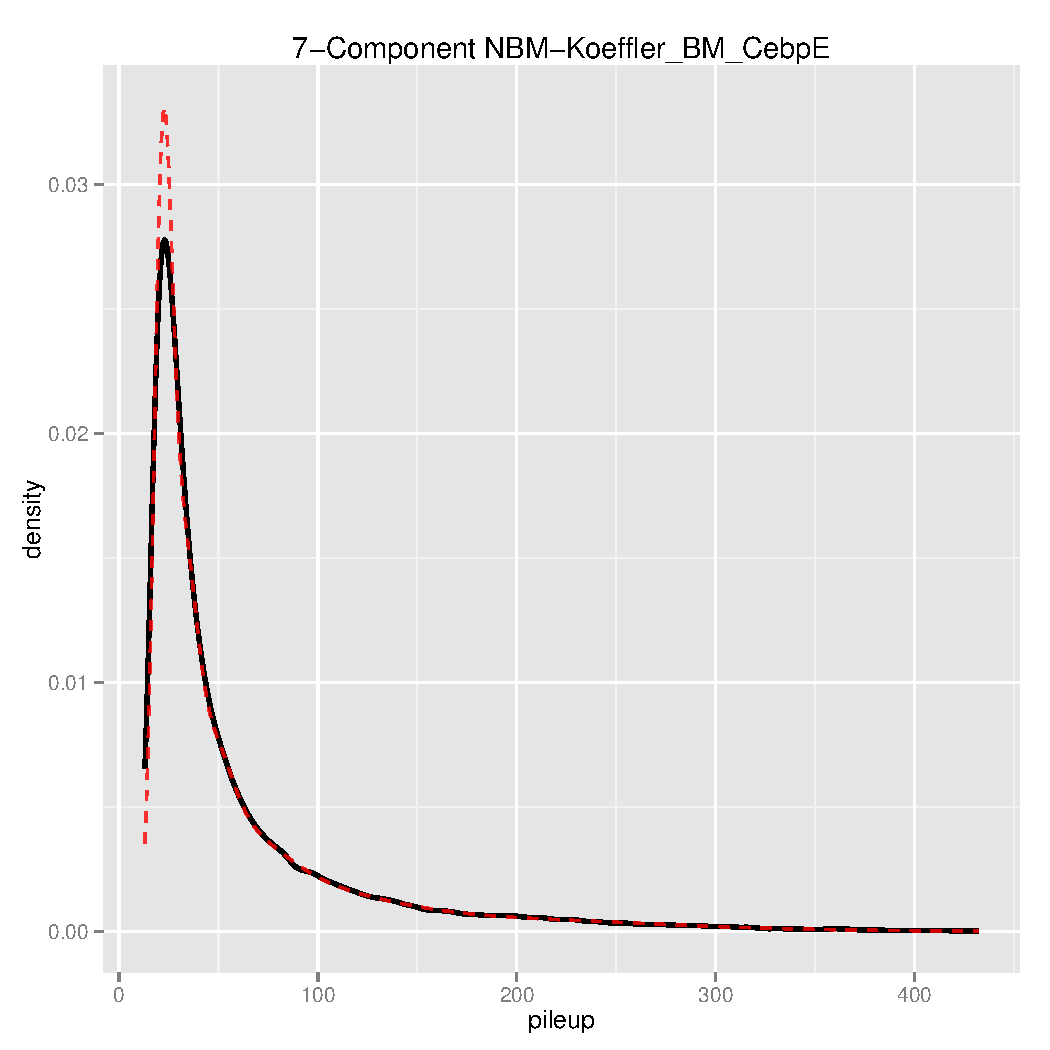
\includegraphics[width = 2in]{figs/Koeffler_BM_CebpE_NBM_ModelVisualization_comp7_empVsModel.pdf}}
    \\
    \subfloat{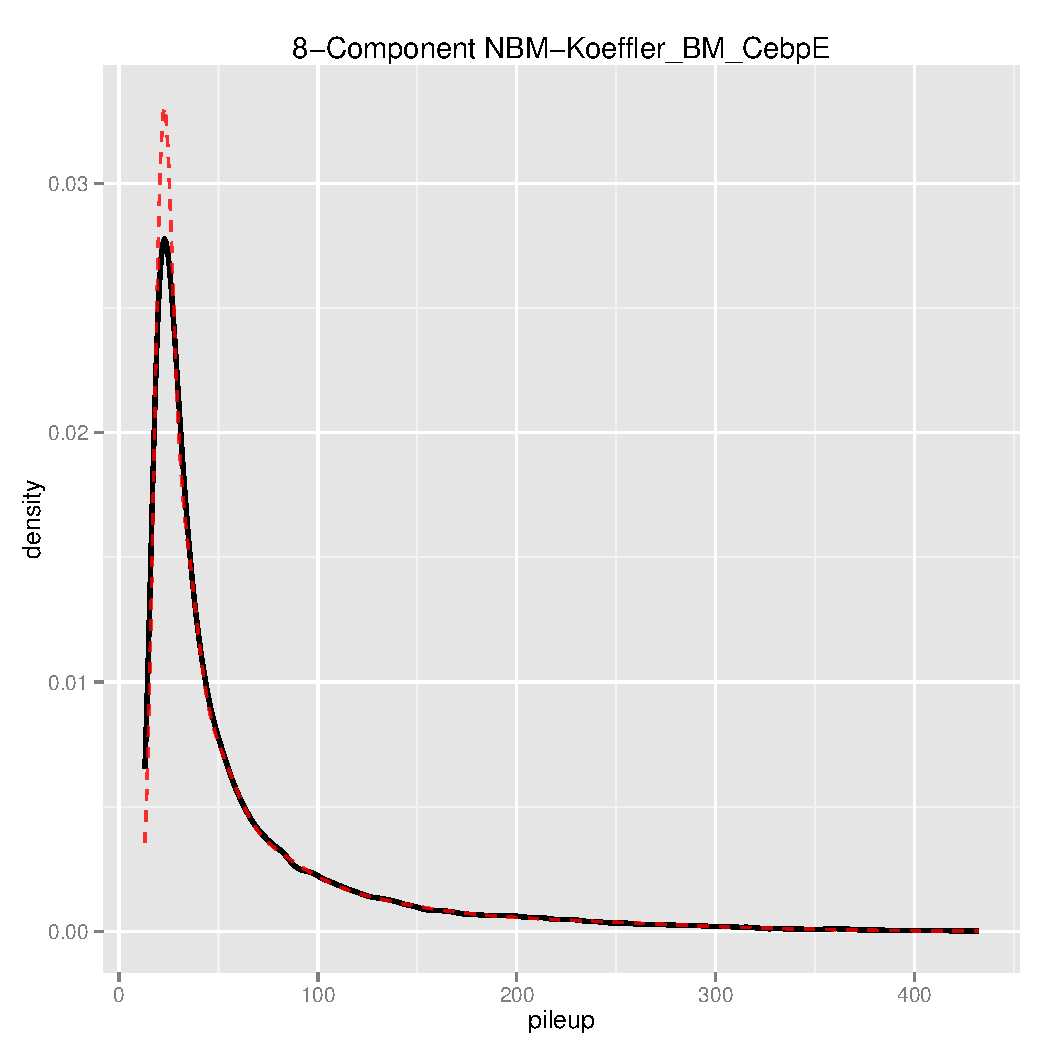
\includegraphics[width = 2in]{figs/Koeffler_BM_CebpE_NBM_ModelVisualization_comp8_empVsModel.pdf}}
    \subfloat{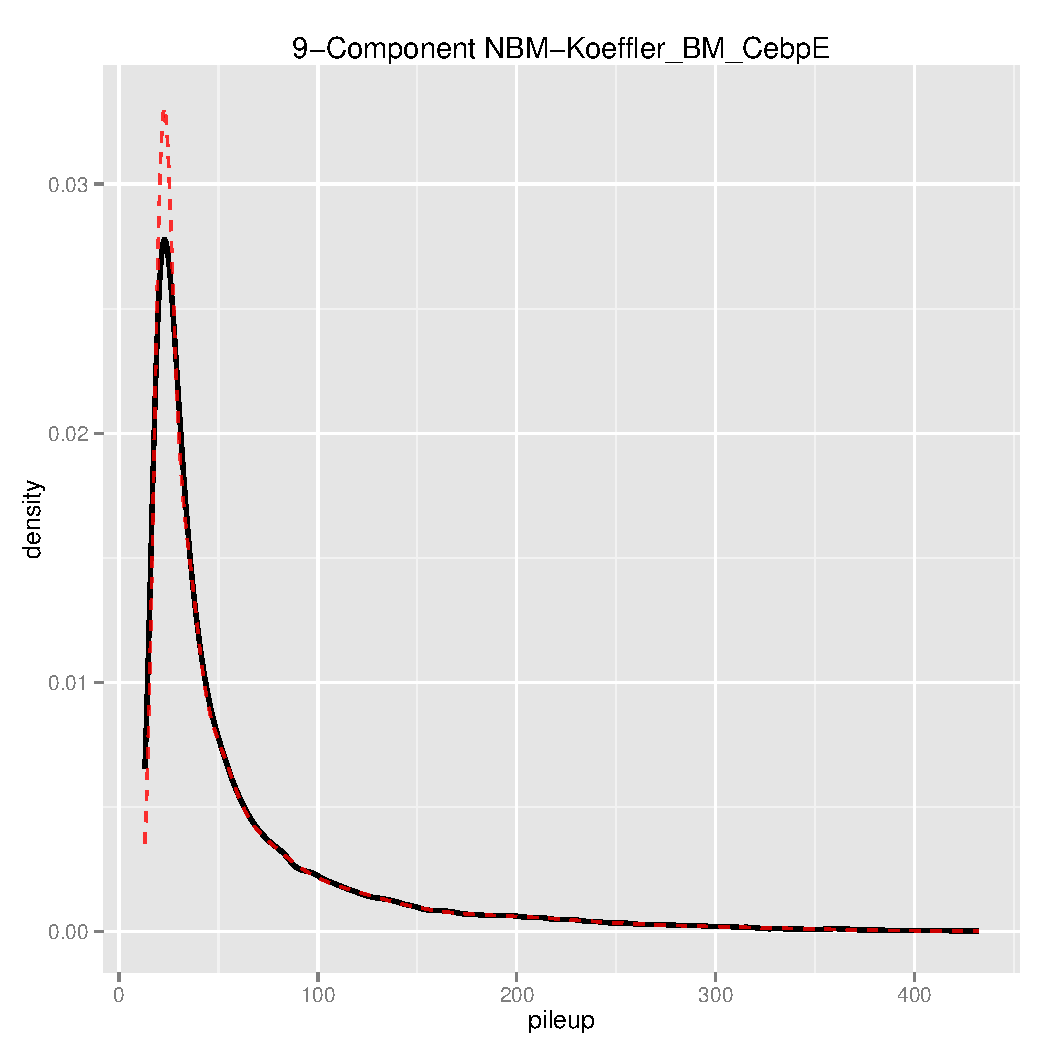
\includegraphics[width = 2in]{figs/Koeffler_BM_CebpE_NBM_ModelVisualization_comp9_empVsModel.pdf}}
    \subfloat{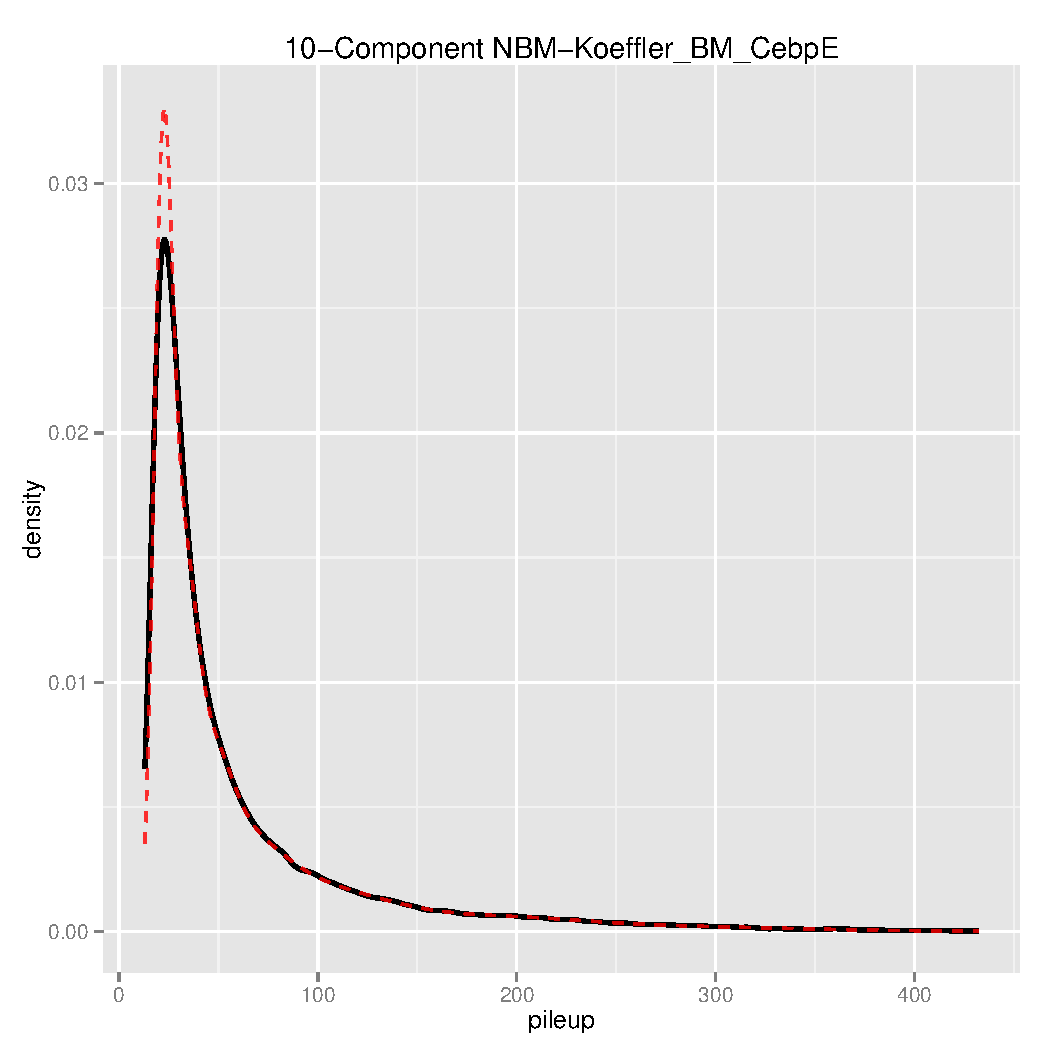
\includegraphics[width = 2in]{figs/Koeffler_BM_CebpE_NBM_ModelVisualization_comp10_empVsModel.pdf}}
    \caption{Comparing Density Estimates: Empirical Vs Gaussian Mixture. Empirical and gaussian density are coloured with black and dashed-red, respectively.}
    \label{fig:empVsnb}
\end{figure}
\clearpage

\section{Stability of the Distribution of Component Assignments}
Here, we checked the distribution of component assignments from 3 different runs (simulation) in order to assess the stability of the fitting models.

Stable component assignment assumes that the number for each component in the course of three different runs stays constant.

\subsection{Stability of the Distribution of Component Assignments: GMMs}





\begin{figure}[H]
    \centering
    \subfloat{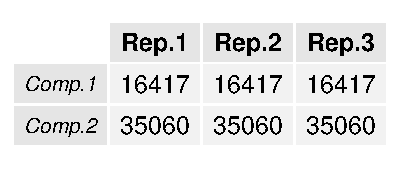
\includegraphics[width = 1.3in, height = 1in]{figs/Koeffler_BM_CebpE_CompFreqTable_2_comp_GMM.pdf}}
    \subfloat{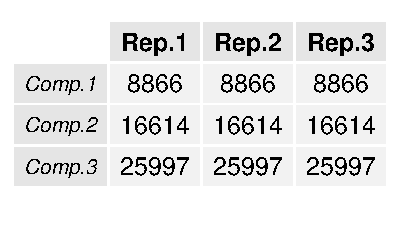
\includegraphics[width = 1.3in, height = 1in]{figs/Koeffler_BM_CebpE_CompFreqTable_3_comp_GMM.pdf}}
    \subfloat{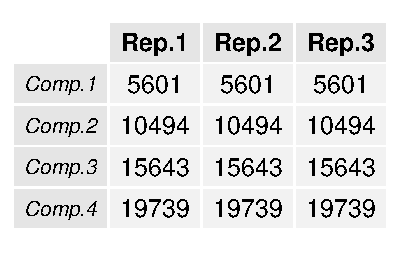
\includegraphics[width = 1.3in, height = 1in]{figs/Koeffler_BM_CebpE_CompFreqTable_4_comp_GMM.pdf}}
    \\
    \subfloat{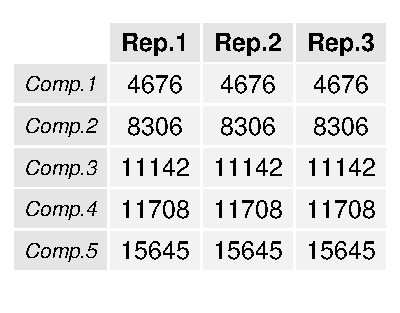
\includegraphics[width = 1.3in, height = 1in]{figs/Koeffler_BM_CebpE_CompFreqTable_5_comp_GMM.pdf}}
    \subfloat{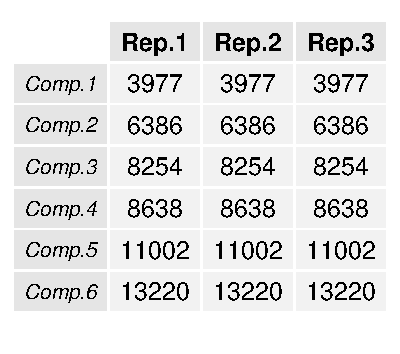
\includegraphics[width = 1.3in, height = 1in]{figs/Koeffler_BM_CebpE_CompFreqTable_6_comp_GMM.pdf}}
    \subfloat{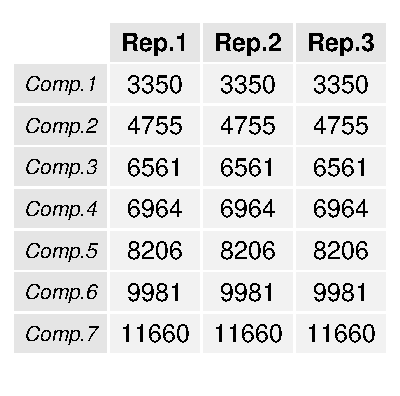
\includegraphics[width = 1.3in, height = 1in]{figs/Koeffler_BM_CebpE_CompFreqTable_7_comp_GMM.pdf}}
    \\
    \subfloat{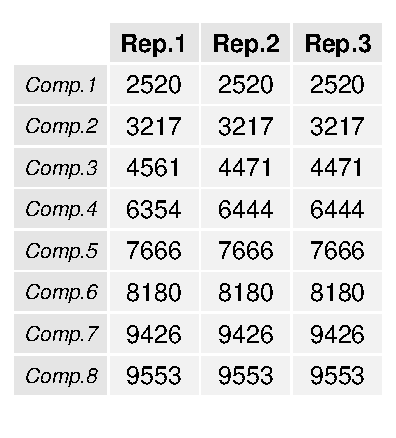
\includegraphics[width = 1.3in, height = 1in]{figs/Koeffler_BM_CebpE_CompFreqTable_8_comp_GMM.pdf}}
    \subfloat{\includegraphics[width = 1.3in, height = 1in]{figs/Koeffler_BM_CebpE_CompFreqTable_9_comp_GMM.pdf}}
    \subfloat{\includegraphics[width = 1.3in, height = 1in]{figs/Koeffler_BM_CebpE_CompFreqTable_10_comp_GMM.pdf}}
    \caption{Component Frequency over Three Different Runs: GMM}
    \label{fig:compFreqGMM}
\end{figure}      

\subsubsection{Stability of the Distribution of Component Assignments: NBMs}




\begin{knitrout}
\definecolor{shadecolor}{rgb}{0.969, 0.969, 0.969}\color{fgcolor}\begin{kframe}
\begin{verbatim}
## pdf pdf pdf pdf 
##   2   2   2   2
\end{verbatim}
\end{kframe}
\end{knitrout}

Note: Fitting with mixture negative binomial from seven components onwards does not assign the whole components for each ChiPseq peaks. For example, with 7-component NBMs, the components assigned are 1,2,3,4,5,6 but not 7. 

\begin{knitrout}
\definecolor{shadecolor}{rgb}{0.969, 0.969, 0.969}\color{fgcolor}\begin{kframe}
\noindent
\ttfamily
\hlstd{}\hlslc{\#\ to\ adjust\ the\ margin\ of\ the\ pdf\ table\ }\hspace*{\fill}\\
\hlstd{}\hlslc{\#for\ f\ in\ \$(ls\ Koeffler\textunderscore BM\textunderscore CebpE\textunderscore CompFreqTable\textunderscore {*});\ do\ pdfcrop\ {-}{-}margins\ '5\ 10\ 5\ 20'\ \$f\ \$f;\ done}\hlstd{}\hspace*{\fill}
\mbox{}
\normalfont
\normalsize
\end{kframe}
\end{knitrout}
 \begin{figure}[H]                                                                                                   \centering
    \subfloat{\includegraphics[width = 1.3in, height = 1in]{figs/Koeffler_BM_CebpE_CompFreqTable_2_comp_NBM.pdf}}
    \subfloat{\includegraphics[width = 1.3in, height = 1in]{figs/Koeffler_BM_CebpE_CompFreqTable_3_comp_NBM.pdf}}
    \subfloat{\includegraphics[width = 1.3in, height = 1in]{figs/Koeffler_BM_CebpE_CompFreqTable_4_comp_NBM.pdf}}
    \subfloat{\includegraphics[width = 1.3in, height = 1in]{figs/Koeffler_BM_CebpE_CompFreqTable_5_comp_NBM.pdf}}
    %\subfloat{\includegraphics[width = 1.3in, height = 1in]{figs/Koeffler_BM_CebpE_CompFreqTable_6_comp_NBM.pdf}}
    \caption{Component Frequency over Three Different Runs: NBM}
    \label{fig:compFreqNBM}
\end{figure}

\section{Model Assessment: Information Criterion}
We assessed the model on the basis of information criterion consisting of AIC (Akaike Information Criterion), BIC (Bayesian Information Criterion), and log-likelihood.\\

We expect the log-likelihood to be increasing as the number of components of GMMs fitted or the negative log-likelihood to be decreasing with increasing number of components.\\

AIC and BIC is based on Occam's razor principle, i.e, the simplest the better. 
As the assessment matrix, AIC and BIC would include the positive contribution of likelihood and also penalize the increasing number of parameters used to fit the model.

The equations of AIC and BIC are as follows:

\begin{flalign}

&AIC = $ -2 \times \log L + 2*P  &&

&BIC = $ -2 \times \log L + \log(n)*P  &&

&$L$ is likelihood &&

&$P$ is the number of parameters &&

\end{flalign}

\subsection{GMMs Model Assessment: AIC and BIC}

\begin{knitrout}
\definecolor{shadecolor}{rgb}{0.969, 0.969, 0.969}\color{fgcolor}\begin{kframe}
\begin{alltt}
\hlkwd{getModelAssessment}\hlstd{(GMMs_list_Koeffler_BM_CebpE,} \hlkwc{max_k} \hlstd{=} \hlnum{10}\hlstd{,}
                   \hlkwc{output_n}\hlstd{=}\hlstr{'figs/Koeffler_BM_CebpE_GMM_ModelAssessment'}\hlstd{,}
                   \hlkwc{model}\hlstd{=}\hlstr{'GMM'}\hlstd{,} \hlkwc{titleName}\hlstd{=}\hlstr{'Koeffler_BM_CebpE'}\hlstd{)}
\end{alltt}
\end{kframe}
\end{knitrout}

\subsection{NBMs Model Assessment: AIC and BIC}

\begin{knitrout}
\definecolor{shadecolor}{rgb}{0.969, 0.969, 0.969}\color{fgcolor}\begin{kframe}
\begin{alltt}
\hlkwd{getModelAssessment}\hlstd{(NBMs_list_Koeffler_BM_CebpE,} \hlkwc{max_k} \hlstd{=} \hlnum{10}\hlstd{,}
                   \hlkwc{output_n}\hlstd{=}\hlstr{'figs/Koeffler_BM_CebpE_NBM_ModelAssessment'}\hlstd{,}
                   \hlkwc{model}\hlstd{=}\hlstr{'NBM'}\hlstd{,} \hlkwc{titleName}\hlstd{=}\hlstr{'Koeffler_BM_CebpE'}\hlstd{)}
\end{alltt}
\begin{verbatim}
## pdf 
##   2
\end{verbatim}
\end{kframe}
\end{knitrout}
\begin{figure}[H]                                                                                                   \centering
    \subfloat{\includegraphics[width = 3in, height = 3in]{figs/Koeffler_BM_CebpE_GMM_ModelAssessment_AICBIC.pdf}}
    \subfloat{\includegraphics[width = 3in, height = 3in]{figs/Koeffler_BM_CebpE_NBM_ModelAssessment_AICBIC.pdf}}
    \caption{Gaussian (left) and Neg.Binomial (right) Mixture Models Assessment: AIC, and BIC.
    Note that BIC introduces the larger penalty term ($\log(n)$) compared with AIC ($2$).
    In this assessment, positive penalty term and negative likelihood are applied. 
    Hence, the lower the score the better the fitting of the model while taking into account its complexity.}
    \label{fig:ModelAssessment}
\end{figure}
\clearpage

\section{Component Assignment by Mixture Models}
\subsection{Component Assignment to ChIP-seq Peaks}

\begin{knitrout}
\definecolor{shadecolor}{rgb}{0.969, 0.969, 0.969}\color{fgcolor}\begin{kframe}
\begin{alltt}
\hlkwd{assignComponentMMs}\hlstd{(Koeffler_BM_CebpE, GMMs_list_Koeffler_BM_CebpE,}
                   \hlkwc{output_n}\hlstd{=}\hlkwd{paste0}\hlstd{(work_dir,}
                    \hlstr{'Output/Koeffler_BM_CebpE_GMM_ModelAssignment'}\hlstd{),}
                    \hlkwc{model}\hlstd{=}\hlstr{'GMM'}\hlstd{,} \hlkwc{sort.comp}\hlstd{=}\hlnum{TRUE}\hlstd{)}
\end{alltt}
\end{kframe}
\end{knitrout}

\begin{knitrout}
\definecolor{shadecolor}{rgb}{0.969, 0.969, 0.969}\color{fgcolor}\begin{kframe}
\begin{alltt}
\hlkwd{assignComponentMMs}\hlstd{(Koeffler_BM_CebpE, NBMs_list_Koeffler_BM_CebpE,}
                   \hlkwc{output_n}\hlstd{=}\hlkwd{paste0}\hlstd{(work_dir,}
                    \hlstr{'Output/Koeffler_BM_CebpE_NBM_ModelAssignment'}\hlstd{),}
                   \hlkwc{model}\hlstd{=}\hlstr{'NBM'}\hlstd{,} \hlkwc{sort.comp}\hlstd{=}\hlnum{TRUE}\hlstd{)}
\end{alltt}
\end{kframe}
\end{knitrout}

\section{Visualization Component Assignment}
\subsection{Visualization Component Assignment}
Here, the sorted-5-component GMM and NBM (Figure ~\ref{fig:Sorted4CompGenomicLocation}) are visualized on chr14.


\begin{figure}[H]
    \centering
    \subfloat{\includegraphics[width = 3in, height = 3in]{figs/Koeffler_BM_CebpE_GMM_ModelAssignment_compSorted4.pdf}}
    \subfloat{\includegraphics[width = 3in, height = 3in]{figs/Koeffler_BM_CebpE_NBM_ModelAssignment_compSorted4.pdf}}
    \caption{Sorted-4-Component GMM (left) and NBM (right) assignment on Chr14.}
    \label{fig:Sorted4CompGenomicLocation}
\end{figure}
\clearpage

\section{Score Distribution of Component Assignments}

The score distribution of 5-component GMM and NBM are shown as boxplots (Figure ~\ref{fig:sorted5CompBoxplot})


\begin{figure}[H]
    \centering
    \subfloat{\includegraphics[width = 3in, height = 3in]{figs/Koeffler_BM_CebpE_GMM_ModelAssignment_compSorted4_Boxplot.pdf}}
    \subfloat{\includegraphics[width = 3in, height = 3in]{figs/Koeffler_BM_CebpE_NBM_ModelAssignment_compSorted4_Boxplot.pdf}}
    \caption{Boxplots of ChIP Peak Scores clustered in 4-component GMM (left) and NBM (right)}
    \label{fig:sorted4CompBoxplot}
\end{figure}
\clearpage





\begin{verbatim}
  Filename: chromatinConformation.Rnw
  Working directory: /home/ricky/Rlim/ChromatinConformation/ComponentCalls/CebpE/ComponentAnalysis 
\end{verbatim}

\section{Metainfo}
\begin{knitrout}
\definecolor{shadecolor}{rgb}{0.969, 0.969, 0.969}\color{fgcolor}\begin{kframe}
\begin{alltt}
\hlkwd{sessionInfo}\hlstd{()}
\end{alltt}
\begin{verbatim}
## R version 3.0.2 (2013-09-25)
## Platform: x86_64-pc-linux-gnu (64-bit)
## 
## locale:
##  [1] LC_CTYPE=en_SG.UTF-8       LC_NUMERIC=C              
##  [3] LC_TIME=en_SG.UTF-8        LC_COLLATE=en_SG.UTF-8    
##  [5] LC_MONETARY=en_SG.UTF-8    LC_MESSAGES=en_SG.UTF-8   
##  [7] LC_PAPER=en_SG.UTF-8       LC_NAME=C                 
##  [9] LC_ADDRESS=C               LC_TELEPHONE=C            
## [11] LC_MEASUREMENT=en_SG.UTF-8 LC_IDENTIFICATION=C       
## 
## attached base packages:
## [1] grid      parallel  stats     graphics  grDevices utils     datasets 
## [8] methods   base     
## 
## other attached packages:
##  [1] plyr_1.8.1           gridExtra_0.9.1      broom_0.2           
##  [4] wordcloud_2.5        BSgenome_1.30.0      Biostrings_2.30.1   
##  [7] rtracklayer_1.22.7   GenomicRanges_1.14.4 XVector_0.2.0       
## [10] IRanges_1.20.7       BiocGenerics_0.8.0   ggbio_1.10.16       
## [13] RColorBrewer_1.0-5   scales_0.2.4         xtable_1.7-3        
## [16] reshape2_1.4         ggplot2_1.0.0        mixtools_1.0.2      
## [19] segmented_0.4-0.0    MASS_7.3-34          boot_1.3-11         
## [22] knitr_1.6           
## 
## loaded via a namespace (and not attached):
##  [1] AnnotationDbi_1.24.0     Biobase_2.22.0          
##  [3] biomaRt_2.18.0           biovizBase_1.10.8       
##  [5] bitops_1.0-6             cluster_1.15.2          
##  [7] codetools_0.2-9          colorspace_1.2-4        
##  [9] DBI_0.2-7                dichromat_2.0-0         
## [11] digest_0.6.4             evaluate_0.5.5          
## [13] formatR_1.0              Formula_1.1-2           
## [15] GenomicFeatures_1.14.5   gtable_0.1.2            
## [17] highr_0.3                Hmisc_3.14-4            
## [19] labeling_0.3             lattice_0.20-29         
## [21] latticeExtra_0.6-26      munsell_0.4.2           
## [23] proto_0.3-10             Rcpp_0.11.2             
## [25] RCurl_1.95-4.3           Rsamtools_1.14.3        
## [27] RSQLite_0.11.4           slam_0.1-32             
## [29] splines_3.0.2            stats4_3.0.2            
## [31] stringr_0.6.2            survival_2.37-7         
## [33] tcltk_3.0.2              tools_3.0.2             
## [35] VariantAnnotation_1.8.13 XML_3.98-1.1            
## [37] zlibbioc_1.8.0
\end{verbatim}
\end{kframe}
\end{knitrout}

\begin{knitrout}
\definecolor{shadecolor}{rgb}{0.969, 0.969, 0.969}\color{fgcolor}\begin{kframe}
\begin{alltt}
\hlkwd{library}\hlstd{(knitr)}
\hlkwd{purl}\hlstd{(}\hlstr{"componentAnalysis.Rnw"} \hlstd{)} \hlcom{# compile to tex}
\end{alltt}
\begin{verbatim}
## [1] "componentAnalysis.R"
\end{verbatim}
\begin{alltt}
\hlkwd{purl}\hlstd{(}\hlstr{"componentAnalysis.Rnw"}\hlstd{,} \hlkwc{documentation} \hlstd{=} \hlnum{0}\hlstd{)} \hlcom{# extract R code only}
\end{alltt}
\begin{verbatim}
## [1] "componentAnalysis.R"
\end{verbatim}
\begin{alltt}
\hlkwd{knit2pdf}\hlstd{(}\hlstr{"componentAnalysis.Rnw"}\hlstd{)}
\end{alltt}


{\ttfamily\noindent\bfseries\color{errorcolor}{\#\# Error: duplicate label 'setup'}}\end{kframe}
\end{knitrout}

\end{document}
